\documentclass[a4paper,11pt]{article}
\usepackage{hyperref,color,url,alltt,parskip,a4wide,array,natbib,booktabs}
%\usepackage{Sweave}
\usepackage{graphicx}
\graphicspath{{../../vignettegraphics/}}
\newcommand{\code}[1]{\texttt{#1}}
\newcommand{\pkg}[1]{\textbf{#1}}
\newcommand{\var}[1]{\emph{#1}}
\newcommand{\link}[1]{#1}
\newcommand{\sQuote}[1]{`#1'}
\newcommand{\setfontsize}[1]{\fontsize{#1}{#1}\selectfont}
\newenvironment{smallexample}{\begin{alltt}\scriptsize}{\end{alltt}}
\newenvironment{example}{\begin{alltt}\small}{\end{alltt}}

\usepackage{color}
\definecolor{Blue}{rgb}{0,0,0.8}
\hypersetup{%
colorlinks,%
plainpages=true,%
linkcolor=black,%
citecolor=black,%
urlcolor=Blue,%
linktocpage=true,%
bookmarksnumbered=true,%
pdfstartview==FitW,%
pdfview={XYZ null null null},%
%pdfpagemode=UseNone,%
pdfauthor={Torben Tvedebrink},%
pdftitle={DNA mixture separation using mixsep}%
}

\begin{document}

%\VignetteIndexEntry{DNA mixture separation}
%\VignetteDepends{mixsep}
%\VignetteKeywords{DNA mixtures}
%\VignettePackage{mixsep}

%\SweaveOpts{engine=R,eps=FALSE}

\title{DNA mixture separation using \pkg{mixsep}}
\author{Torben Tvedebrink\\
  Department of Mathematical Sciences\\ Aalborg University\\
  \url{tvede@math.aau.dk}
}
\maketitle
\sloppy

\noindent This vignette describes how the \pkg{mixsep} can be used to
separate DNA mixtures of two and three DNA profiles. The implemented
algorithm is based on the research paper by \cite{tvedebrink2011}. For
more details and motivation please see that paper. 

\textbf{DISCLAIMER:} \textsl{This vignette is not completely
  up-to-date compared to version of \pkg{mixsep} available at CRAN. It
  is expected to be fixed during July/August of 2011.}

\section{Create a desktop shortcut (Windows only)}
\label{sec:shortcut}

When \textsf{R} and \pkg{mixsep} are installed the
\code{makeShortcut}-function in the \pkg{mixsep}-package can be used
to create a shortcut on the Windows desktop. 

There are several reasons to do so: 
\begin{itemize}
\item Makes it easier and faster to start the \pkg{mixsep} GUI.
\item The performance of tcl/tk within R is improved when it is run
  outside the RGui.
\item If the \code{makeShortcut}-function is given a configuration
  file a database connection is readily available by start-up (see
  Section~\ref{sec:db} for further details).
\end{itemize}

In Figure~\ref{fig:shortcut} a screen short of the RGui after the
\pkg{mixsep}-package is loaded and the \code{makeShortcut}-function is
executed. Note that in order to call \code{library(mixsep)}
successfully the package needs to be available/installed in
\textsf{R}. If no errors occur a shortcut icon to \pkg{mixsep}
(similar to the one in Figure~\ref{fig:shortcut}) is created on the
Windows desktop.

\begin{figure}[!h]
  \centering
  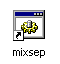
\includegraphics{shortcut_icon}
  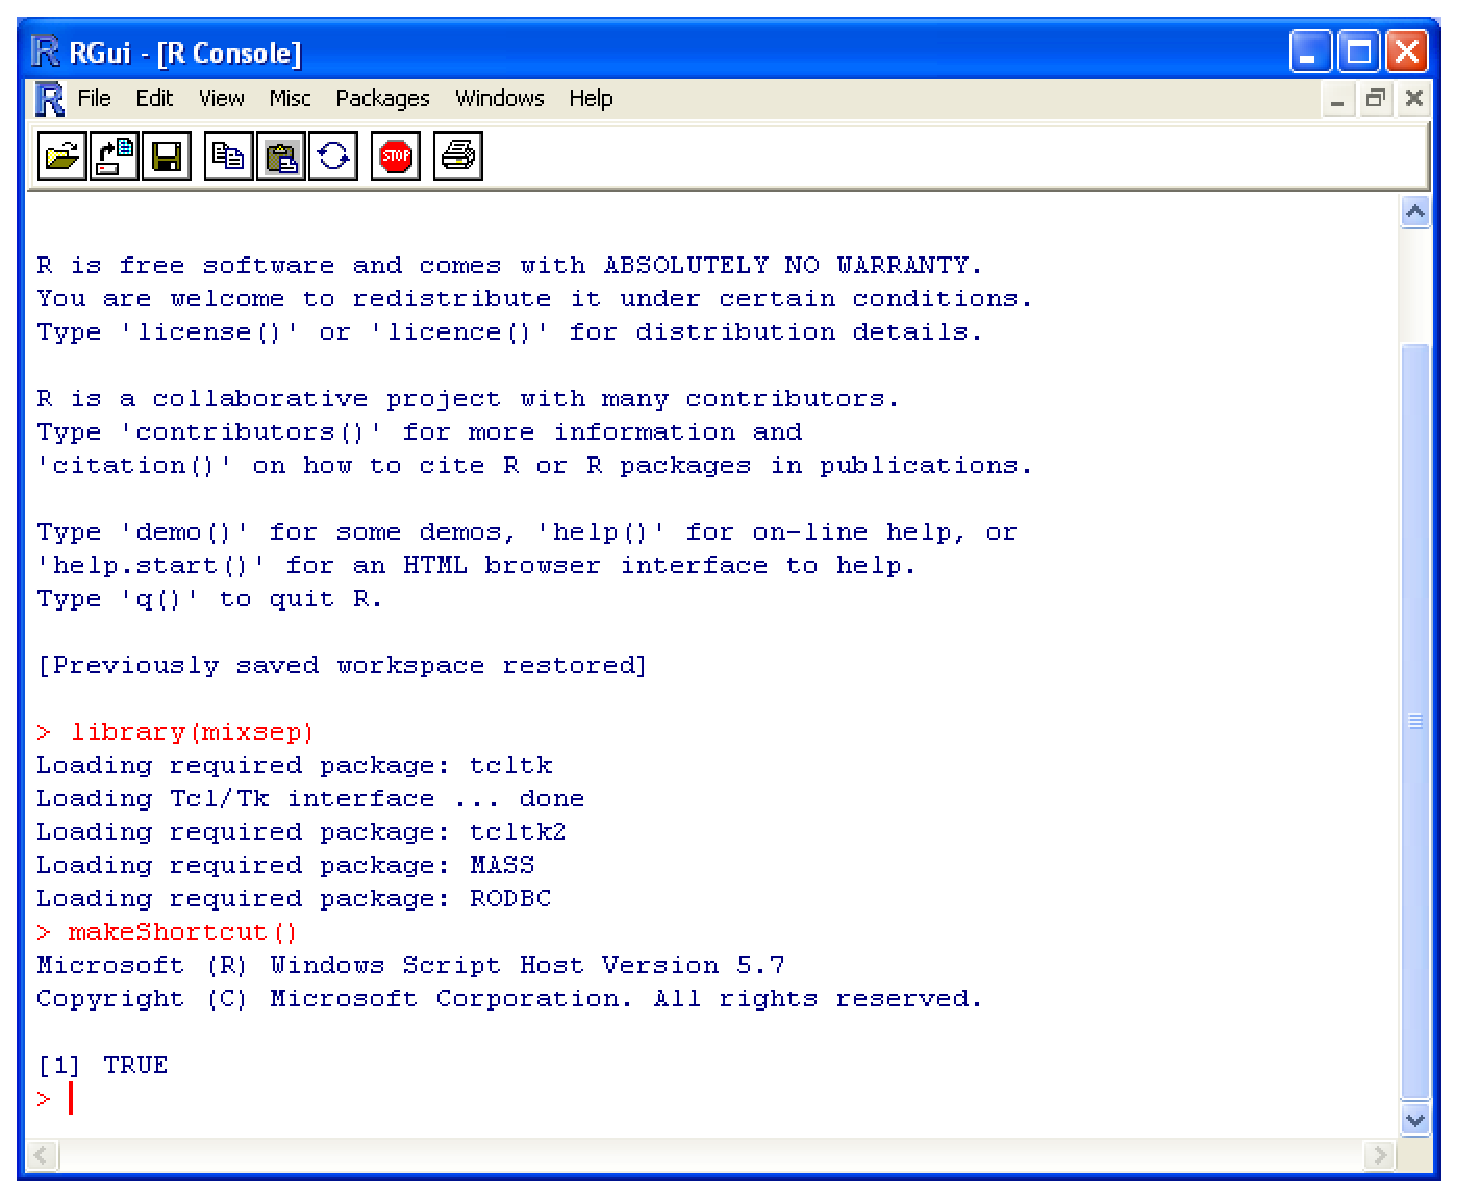
\includegraphics[width=10cm]{shortcut_make}
  \caption{\label{fig:shortcut}Shortcut creating under \textsf{R} for
    Windows}
\end{figure}


\section{Database connection and data extraction}
\label{sec:db}

\subsection{Setting up data connection to a database}
\label{sec:setup-db}

Because \pkg{mixsep} depends on the \pkg{RODBC}-package it is
possible to connect to a database and retrieve case information data
without an intermediate create/read file step.

In order to do so one needs to give a connection file as argument to
the \code{makeShortcut}-function (see the
Section~\ref{sec:shortcut}). One example of such a file is given below
(the file name and extension is unimportant). The \pkg{mixsep} GUI
uses the \code{odbcDriverConnect}-function from the
\pkg{RODBC}-package in order to connect to a database. Hence, please
refer to the documentation for this function by typing
\code{?odbcDriverConnect} in \textsf{R} or read the package
\href{http://cran.r-project.org/web/packages/RODBC/vignettes/RODBC.pdf}{Vignette}
by Brian Ripley.

The content of connection file (\code{tvede.connect}). It is
important that only one argument (\code{db, dbtab,
dbcase, dbcols}) is specified per line. Each argument is given
in double-quotes (\code{"argument"}) and these are
separated by semi-colon (\code{"argument1;
argument2"}). Each line is described in more detail below:

\begin{example}
## Settings for connecting to the MySQL server on Torben Tvedebrink's laptop 
db = "DSN=mixsepServer; Database=mixsep"
dbtab = "samples"
dbcase = "cases"
dbcols = "replicate; fraction"
\end{example}

\textbf{db}\quad
The \code{db} argument gives the DSN connection
name and specifications to \code{odbcDriverConnect}. In the example above the ODBC
data source is called \code{mixsepServer} and the
particular database \code{mixsep}. 

\textbf{dbtab}\quad
The \code{dbtab} argument specifies which table on
the \code{db} we access, e.g. a possible 
database query is \code{"SELECT * FROM dbtab"}.

\textbf{dbcase}\quad
The \code{dbcase} specifies the column containing
the case number associated with a given case. Note that there may be
several analysis results sharing \code{dbcase}-value if these are e.g. replicate runs,
different PCR fractions, etc.

\textbf{dbcols}\quad
As mentioned under \code{dbcase} can several
analysis result share \code{dbcase}-value. However,
there should at least be one column making it possible to distinct
between these. This/these columns are specified as \code{dbcols}.

The screen short in Figure~\ref{fig:shortcut_db} show the creation of
a mixsep desktop shortcut while creating the database
connection. \textbf{NOTE:} The connection file (here
\code{tvede.connect}) needs to be in the \textsl{current working
  directory}, which is set by selecting ``Change dir...'' under
``File'' in the menu (see Figure~\ref{fig:changedir}). The chosen
directory should contain the connection file.

\begin{figure}[!h]
  \centering
  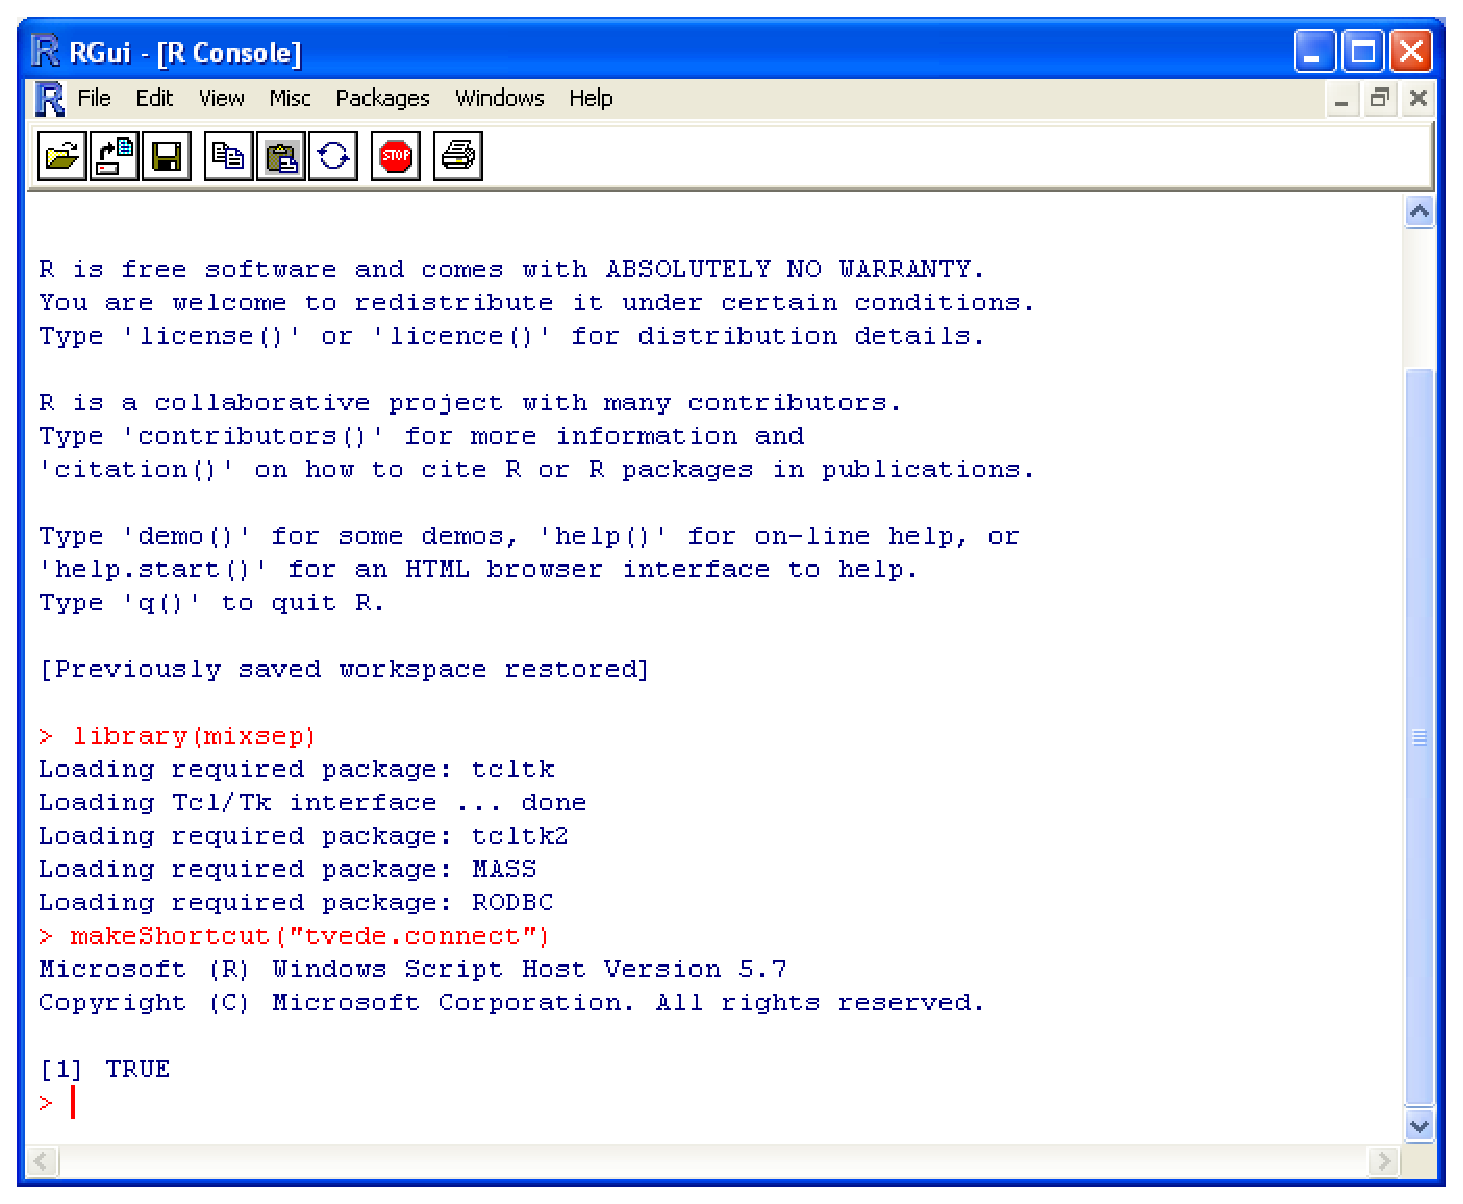
\includegraphics[width=12cm]{shortcut_db}
  \caption{\label{fig:shortcut_db}Creating a shortcut for the Windows
    desktop and setting up a database connection.}
\end{figure}

\subsection{Extract data from a database connection}
\label{sec:extract-db}

By using the shortcut created above a database-button is available on
the ``Files''-tab of the \pkg{mixsep} GUI (Figure~\ref{fig:front}).

\begin{figure}[!h]
  \centering
  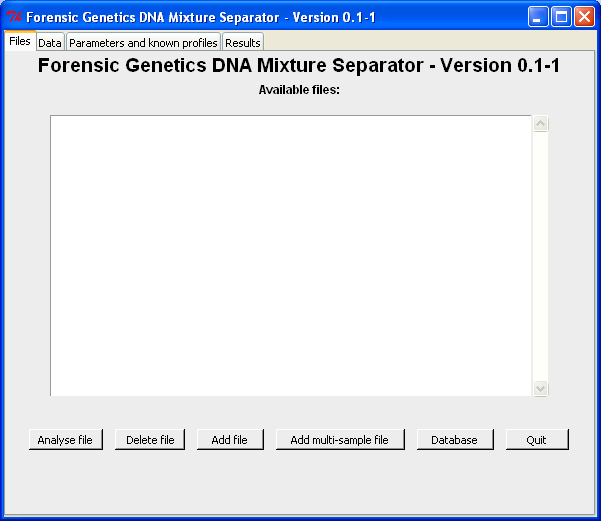
\includegraphics[width=10cm]{front}
  \caption{\label{fig:front}If a database connection is setup the
    Database-button appears on the ``Files''-tab.}
\end{figure}

By clicking this button a ``database query''-window opens in which
queries to the specified database can be made
(Figure~\ref{fig:database_query}). A query is made to the database
matching all entries in the database with \code{dbcase} containing the
specified case identifier. The result is stratified by \code{dbcols}.

In Figure~\ref{fig:database_query} the second screen shot a query to
the case \textsl{10-18687} is made and three different analysis
results are returned (third screen shot of
Figure~\ref{fig:database_query}). Furthermore, the call to the
database uses \textsl{wild cards} such that any consecutive sub-string
of \textsl{10-18687} would yield the three samples (and possibly
more). Note that ``:'' is used to separate the column information from
the columns specified in \code{dbcase} and \code{dbcols} above. Each
row corresponds to an unique sample file (originating from different
replicates and PCR runs).

The sample(s) of interest can be transferred to the main window by
double-click a the row or by highlighting the row(s) and click
``Transfer selected entries''. Note both [Shift], [Ctrl] and [Ctrl-a]
can be used to select more/all samples. Here we select
\textsl{10-18687:2:36\_100824-8.4JPL} for further analysis (which is
then transferred to the main window - see fourth screen shot of
Figure~\ref{fig:database_query}):

\begin{figure}[!h]
  \centering
  \begin{tabular}{cc}
    \parbox{7.5cm}{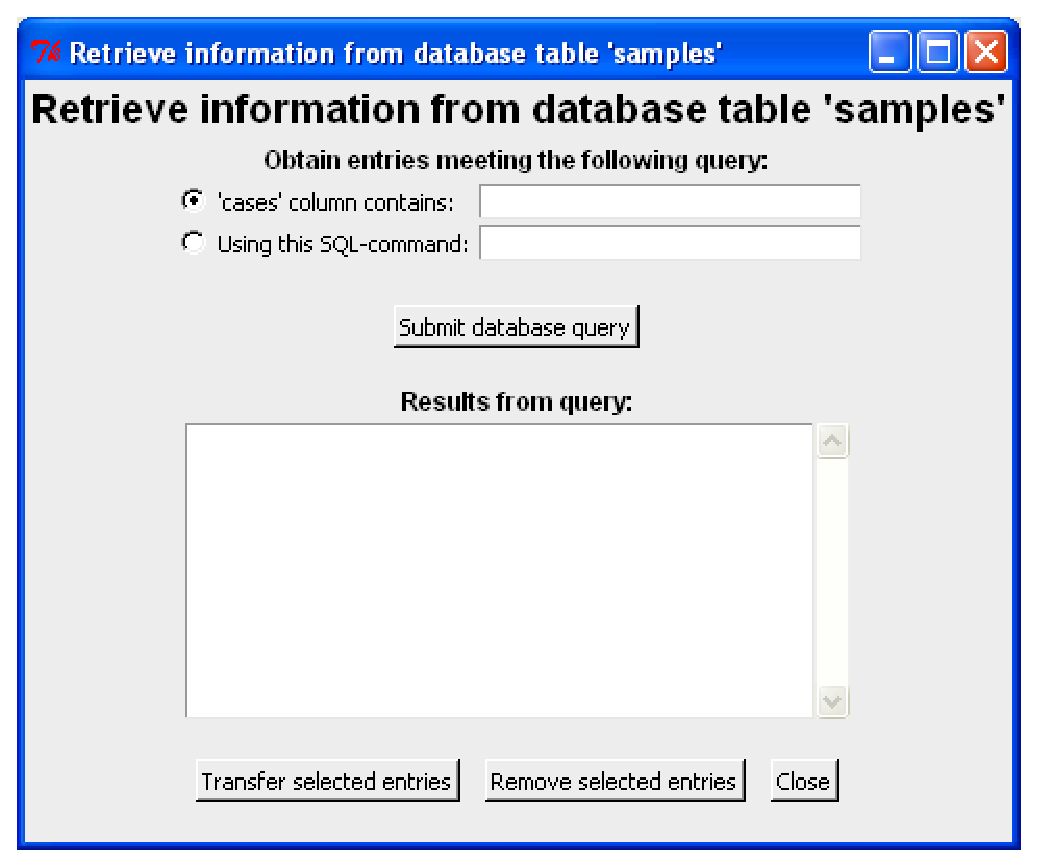
\includegraphics[width=7.4cm]{database_query}} &
    \parbox{7.5cm}{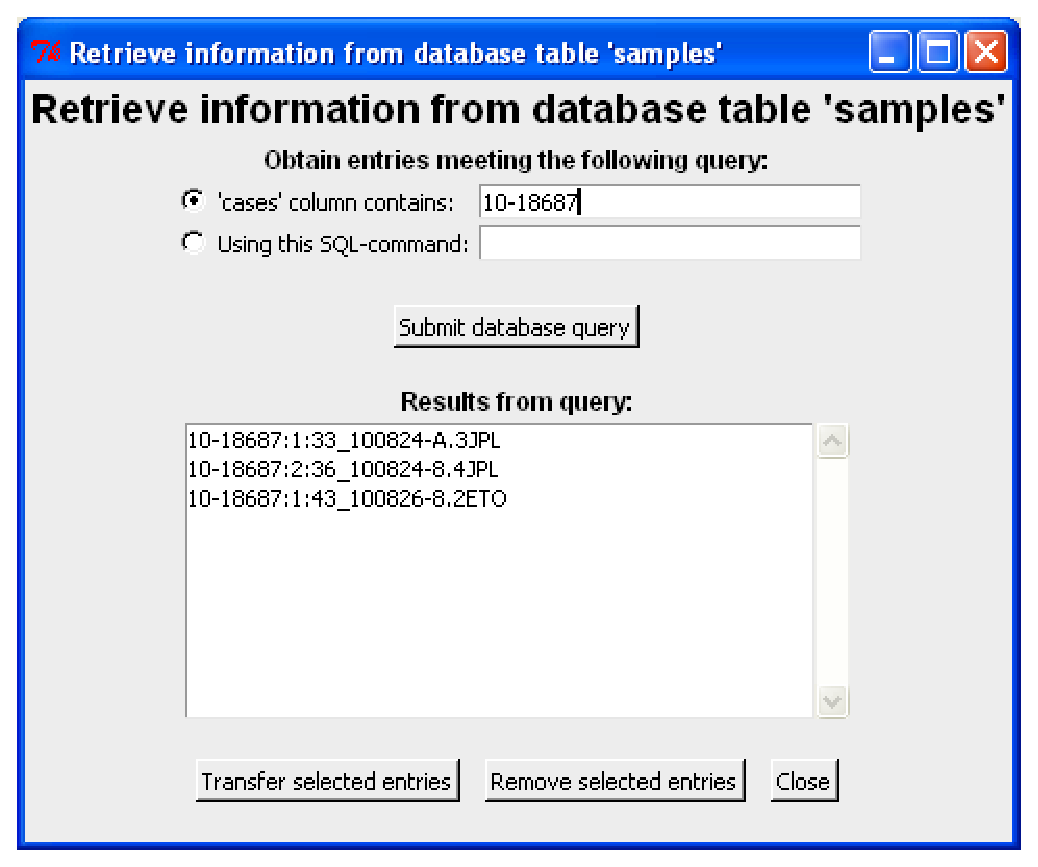
\includegraphics[width=7.4cm]{database_query_result}}\\
    Query window. & Result of \textsl{10-18687} query.\\\\
    \parbox{7.5cm}{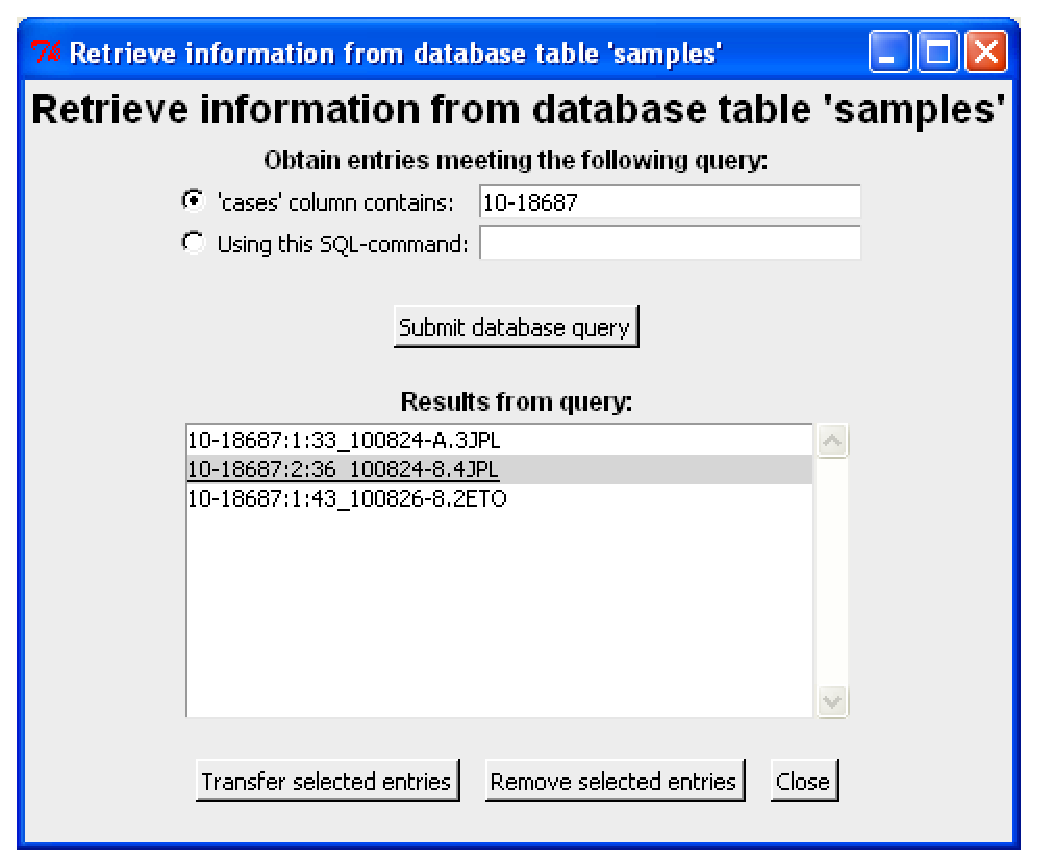
\includegraphics[width=7.4cm]{database_query_select}} &
    \parbox{7.5cm}{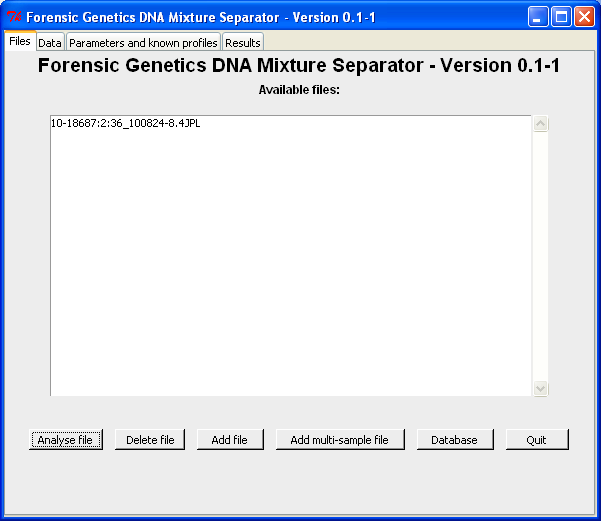
\includegraphics[width=7.4cm]{database_transfer}}\\
    Mark a entry for transfer. & Data transferred to main window.\\
  \end{tabular}
  \caption{\label{fig:database_query}Process of querying the database
    and transfer data to the main window.}
\end{figure}

\section{Load data from files}
\label{sec:files}

\subsection{Load data from file(s) with a single case and replicate}
\label{sec:singlefile}

In order to load data from files these needs to be either .csv-files
(semi-colon separated, \textsl{delimiter: ``;''}, or comma separated,
\textsl{delimiter: ``,''}) or .tab-files (tabular
separated). \textsl{Other formats may be included in later releases if
  requested by the users}.

To load file(s) with a single case (and replicate) use the ``Add
file''-button, which opens a ``Open file''-dialogue window. One or
more files can be selected (Figure~\ref{fig:files}).

\begin{figure}[!h]
  \centering
  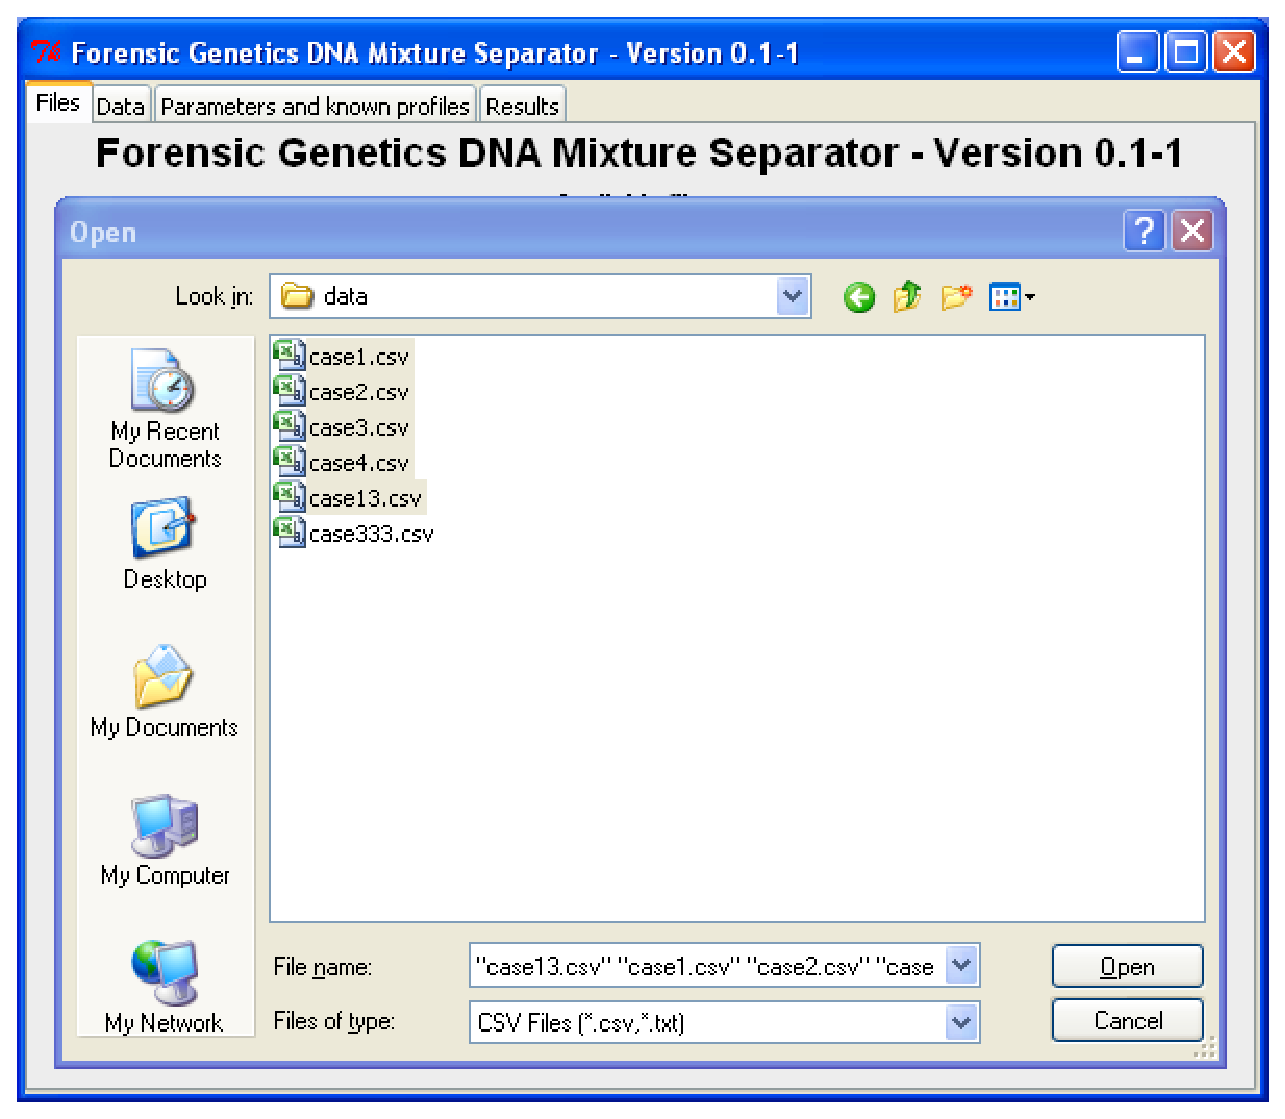
\includegraphics[width=7.4cm]{files_load_multiple_files}
  \quad
  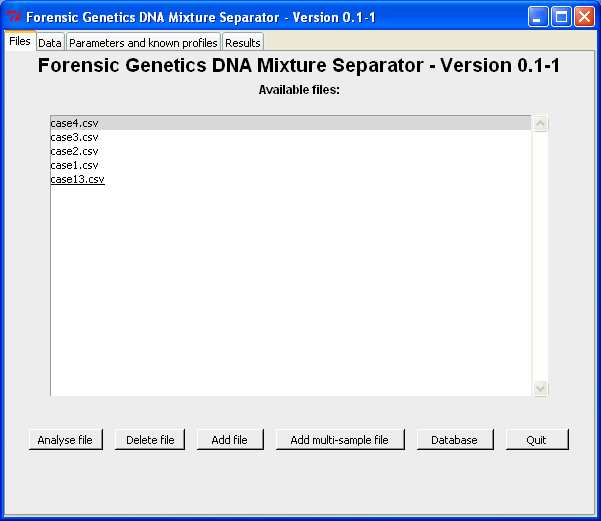
\includegraphics[width=7.4cm]{files_multiple_files}
  \caption{\label{fig:files}Opening several files
    and load of data into main window.}
\end{figure}

After clicking ``Open'' in the dialogue window, the selected file(s) are
present in the ``Available files'' list for further analysis
(Figure~\ref{fig:files}). In Section~\ref{sec:wangbm} it is demonstrated
how a file is analysed.

\subsection{Load data from file(s) with multiple cases/replicates}
\label{sec:multifile}

If a file contains more cases or replicates of the same case, the
``Add multi-sample file''-button should be used. This opens a ``Open
file''-dialogue window, where one or more files can be selected (see
single file description in Section~\ref{sec:singlefile}). However, in
order to specify which columns that uniquely determines the different
samples a second dialogue window opens (top screen shot in
Figure~\ref{fig:multifiles})

\begin{figure}[!h]
  \centering
  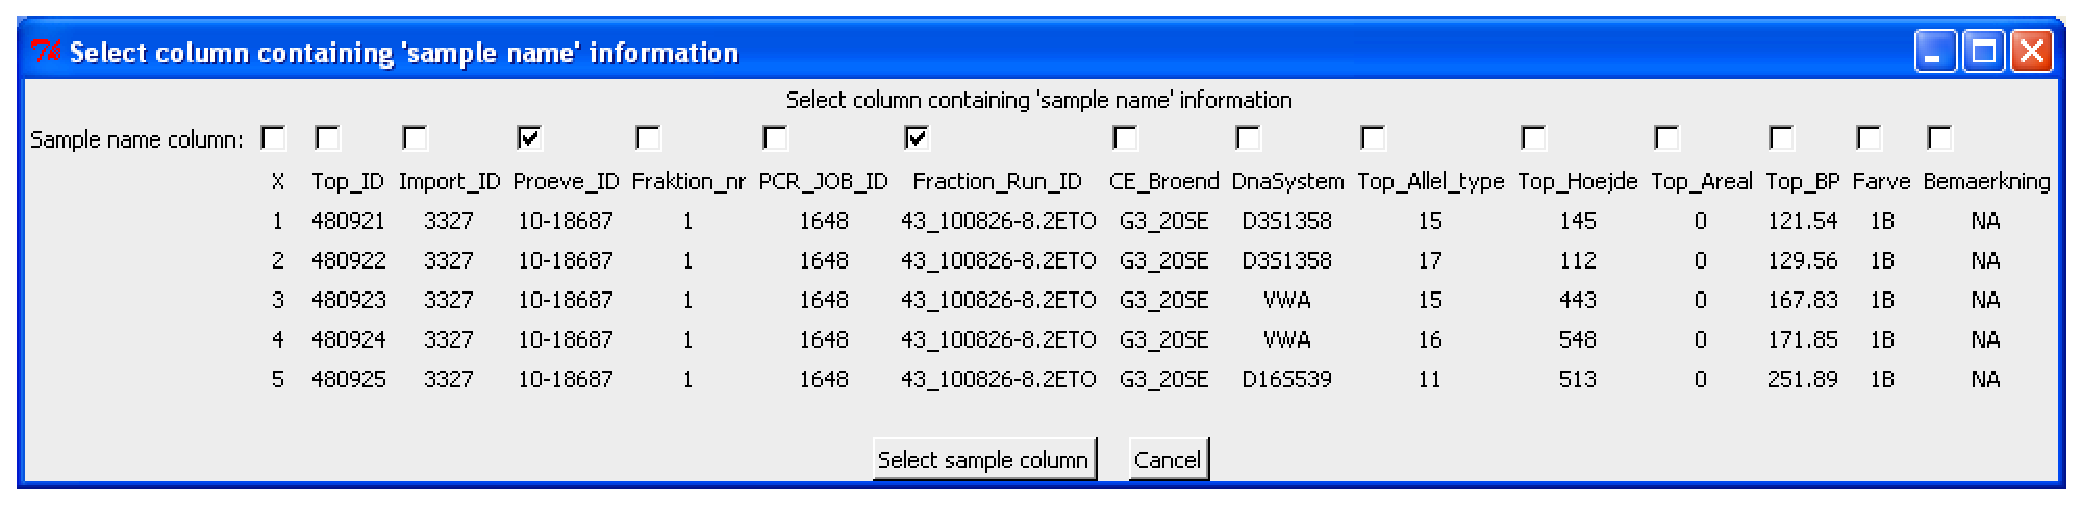
\includegraphics[width=15cm]{multisample}\\\vskip3mm  
  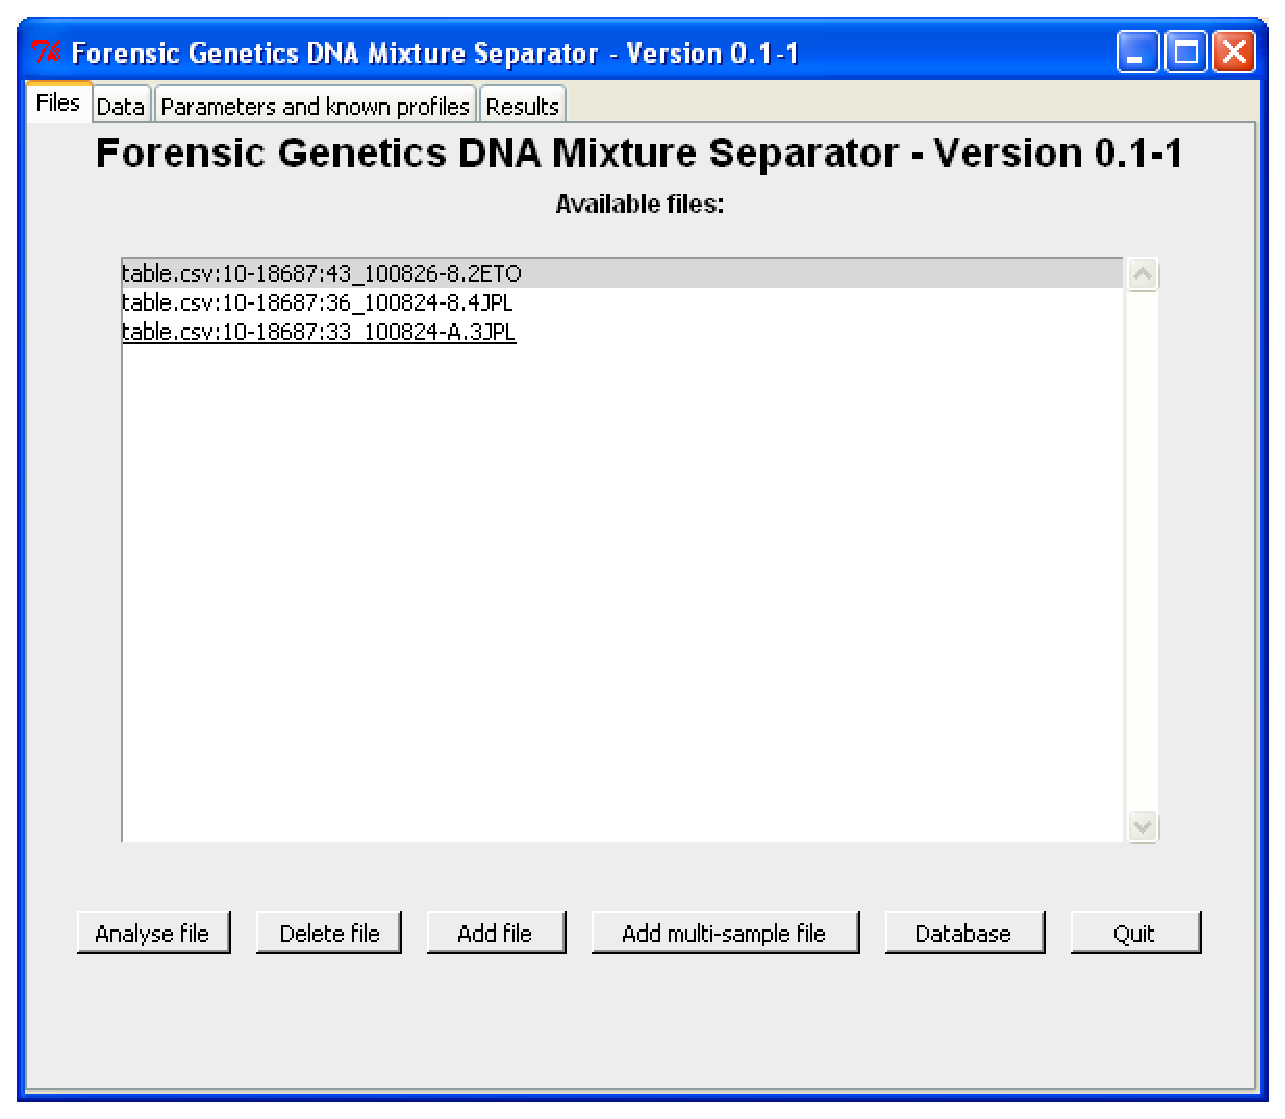
\includegraphics[width=10cm]{files_multisample}
  \caption{\label{fig:multifiles}Multi-sample files loaded into the
    main window.}
\end{figure}

In the top screen shot of Figure~\ref{fig:multifiles} are
\textsl{Proeve\_ID} and \textsl{Fraction\_Run\_ID} selected since
these uniquely separates the rows into three different samples. By
clicking ``Select sample column'' the data is transferred to the main
window. Note that \textsl{Proeve\_ID} is fixed for all samples, but
since this column contain the case number information we also mark
this column (See bottom screen shot of Figure~\ref{fig:multifiles}.

\newpage

\section{Determine the best matching configuration}
\label{sec:wangbm}

We demonstrate how to determine the best matching configuration for a
two-person DNA mixture using the wang.csv-file. This file contains
data previously published by \citet{wang2006}. First we load the file
(as described in Section~\ref{sec:singlefile}) to get the file present
in ``Available files''-list as in Figure~\ref{fig:wangload}.

\begin{figure}[!h]
  \centering
  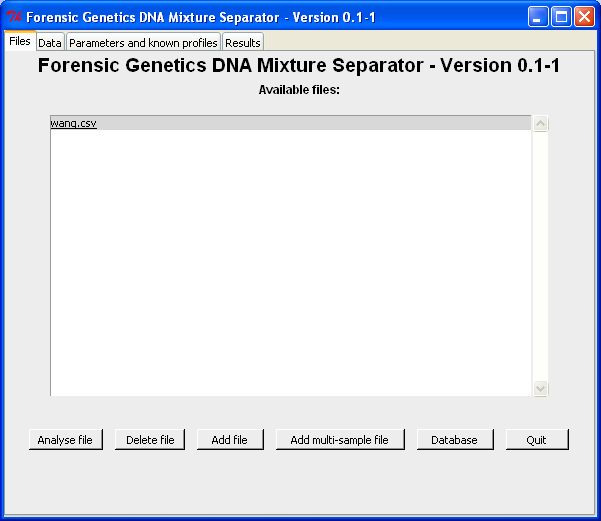
\includegraphics[width=10cm]{files_singlefile}
  \caption{\label{fig:wangload}The tutorial data file ``wang.csv'' is loaded.}
\end{figure}

By marking the file name and click the ``Analyse file''-button (or
double-click on the file name), we obtain the ``Data''-tab shown in
Figure~\ref{fig:datatab}. In the ``Data''-tab the columns containing
the relevant information are selected (left screen shot). Since
wang.csv only contain information about locus, allele and area, we
leave ``Height'', ``bp'' and ``Dye'' empty.

After the columns are selected (by clicking ``Select columns''), we
obtain all the rows (for the selected columns) in the file (right
screen shot of Figure~\ref{fig:datatab}). For each row it is possible
to select/remove the peak from the analysis. However, we recommend
that the removal of rows is used with caution, since all information
should be considered and dealt with!

\begin{figure}[!h]
  \centering
    \begin{tabular}{cc}
      \parbox[b]{7.5cm}{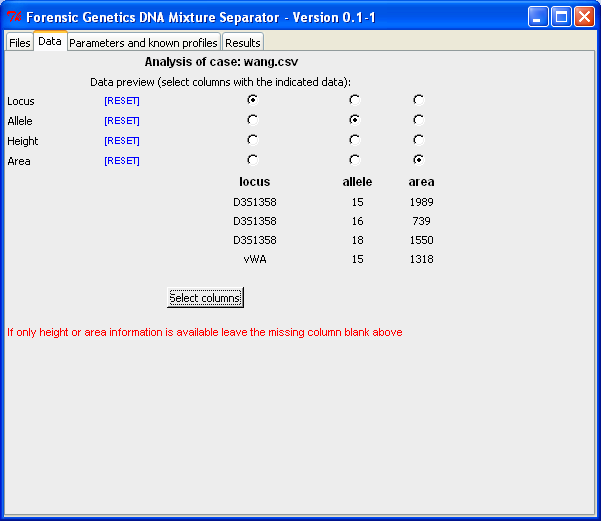
\includegraphics[width=7.5cm]{data_columns}}&
      \parbox[b]{7.5cm}{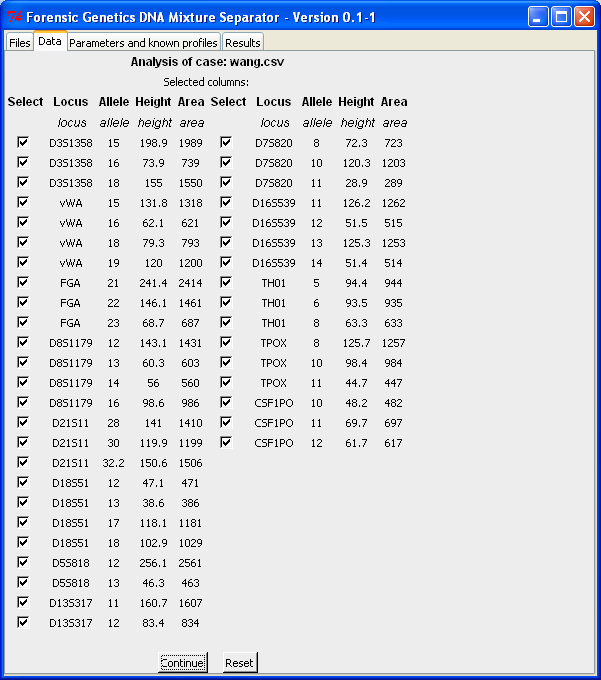
\includegraphics[width=7.5cm]{data_rows}}
      \end{tabular}
  \caption{\label{fig:datatab}The two states of the
    ``data''-tab. Left: Select the relevant columns. Right: Select the
    rows of interest (all rows are selected by default).}
\end{figure}

The ``Parameters and known profiles''-tab makes it possible to specify
the number of contributors, whether the algorithm should search for
alternatives, etc. It is also here that fixed/known profiles can be
specified (see Section~\ref{sec:wangfix} for an analysis with fixed
profiles). From the parameter settings in Figure~\ref{fig:nofixed}, we
assume the sample is a two-person mixture and searches for
alternatives (the lower the level of significance is, the more
alternatives are included in the final result).

\begin{figure}[!h]
  \centering
  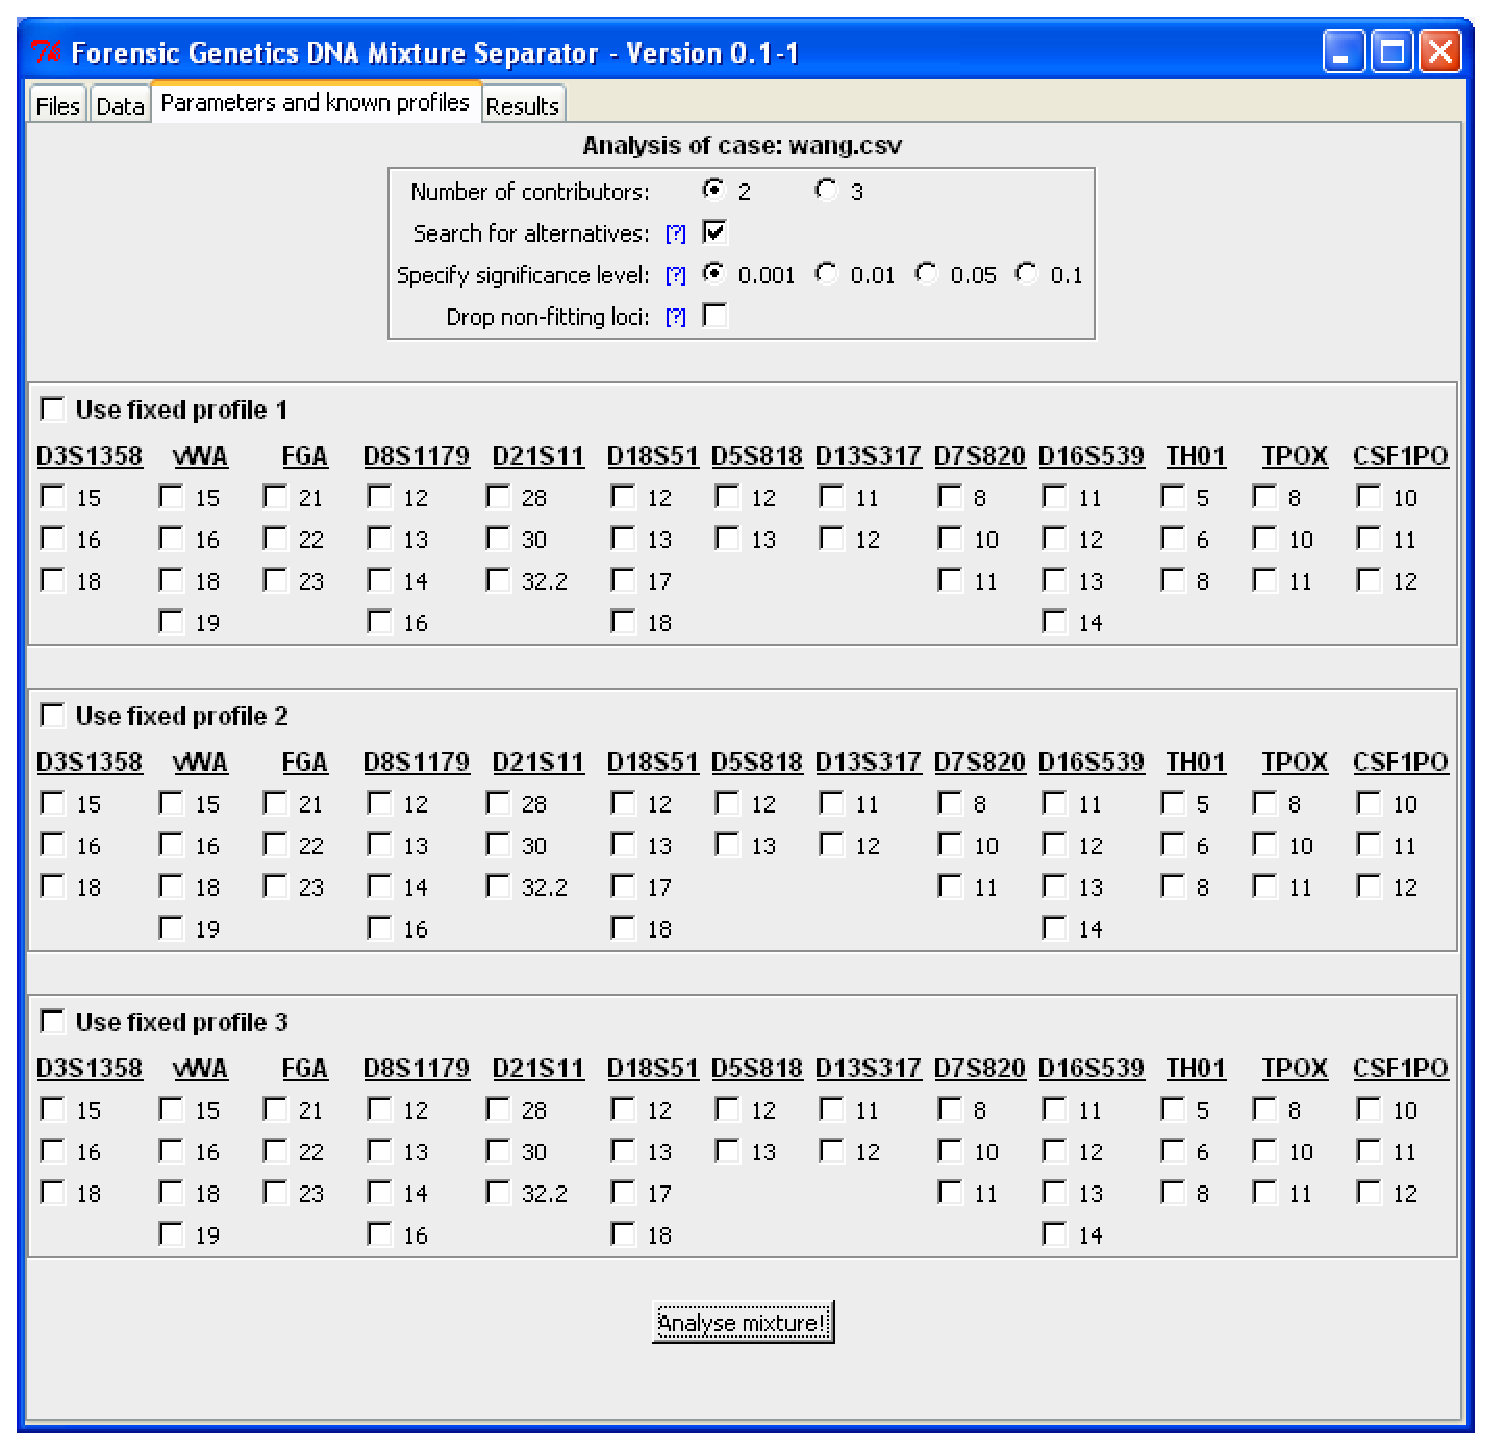
\includegraphics[width=10cm]{param_nofixed}
  \caption{\label{fig:nofixed}Parameter settings implying a two-person
    DNA mixture and search for alternative configurations.}
\end{figure}

When clicking ``Analyse mixture!'' the computer resolves the DNA
mixture and returns result in the
``Result''-tab. Figure~\ref{fig:resultbm} has the output from the
analysis. For each locus a best matching configuration (which is
identical to the true profiles, see by \citet{wang2006}) is identified
together with a list of possible alternatives. Next to the locus
designation is the number of possible alternatives for that locus
given in parenthesis. Below the list of locus configurations is the
number of total configurations given together with the estimated
parameters of the statistical model. The ``Estimated alpha''
represents the mixture proportion of the minor contributor. Here it is
0.3 which corresponds to an 1:2-mixture ratio. The ``Estimated tau''
value represents that residual variance, which means that the smaller
the estimate the better is the concordance between the observed and
expected peak intensities (the ``Derived R\^{}2'' quantity is
explained below).

\begin{figure}[!h]
  \centering
  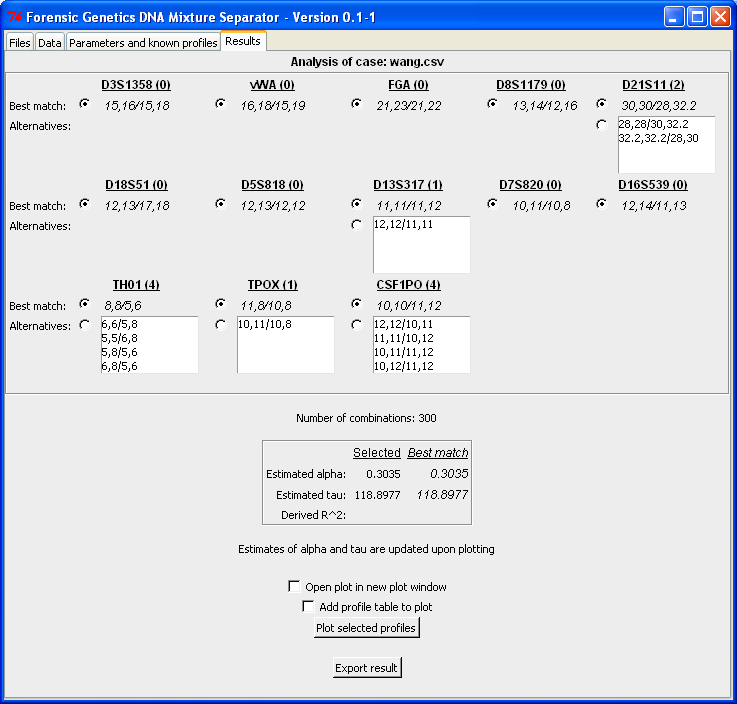
\includegraphics[width=10cm]{result_bestmatch}
  \caption{\label{fig:resultbm}Results from the best matching analysis.}
\end{figure}

The expected peak intensities for the selected configuration can be
plotted against the observed peak intensities in a EPG-like plot
(Figure~\ref{fig:plotbm}). The coloured cones represents the observed
peak intensities, while the black lined cones show the expected peak
intensities (for this particular plot it is hard to see any
discrepancies, which indicate a good fit between the observed and
expected peak intensities).

\begin{figure}[!h]
  \centering
  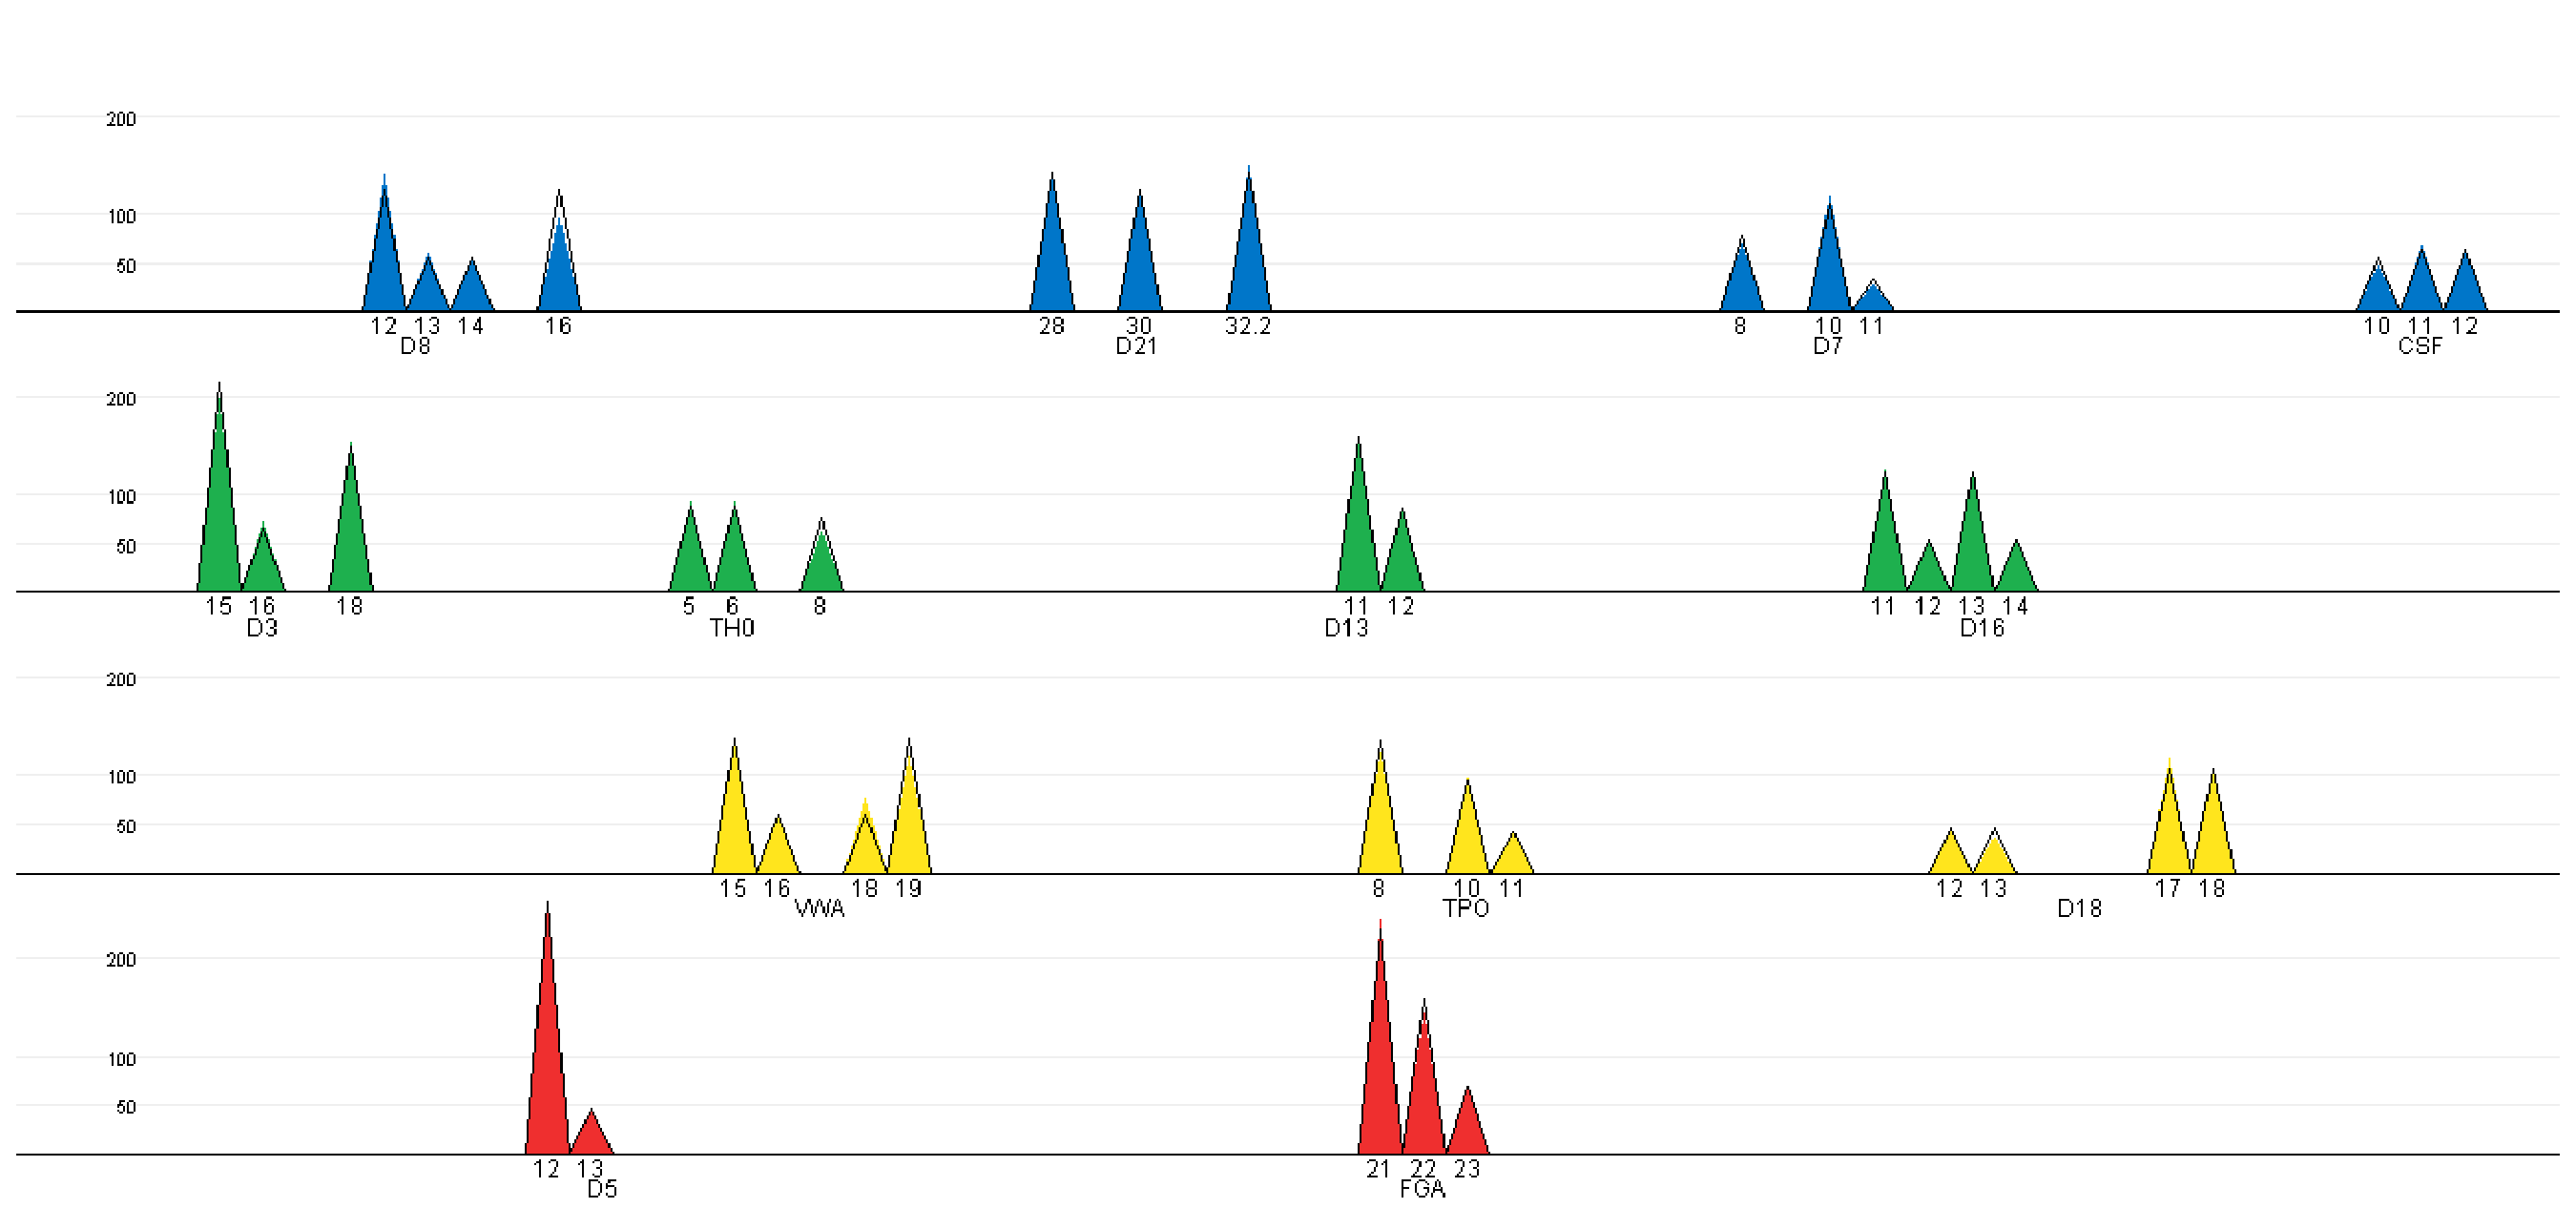
\includegraphics[width=15cm]{plot_bestmatch}
  \caption{\label{fig:plotbm}EPG for the best matching pair of DNA
    profiles. The coloured cones show the observed peak intensities
    whereas the solid black cones represents the expected peak
    intensities.}
\end{figure}

From the analysis output alternative configurations can be specified
by marking the combinations in the lists. For each locus the list of
alternatives is sorted in decreasing order in terms of
goodness-of-fit. For the selected configuration
(Figure~\ref{fig:resultalt}) the R\^{}2-quantity is computed as the
ratio of the estimated tau values. Here R\^{}2 = 0.38 = 118/310 and
the closer R\^{}2 is to 1, the better is the alternative configuration
relative to the best match pair of profiles.

\begin{figure}[!h]
  \centering
  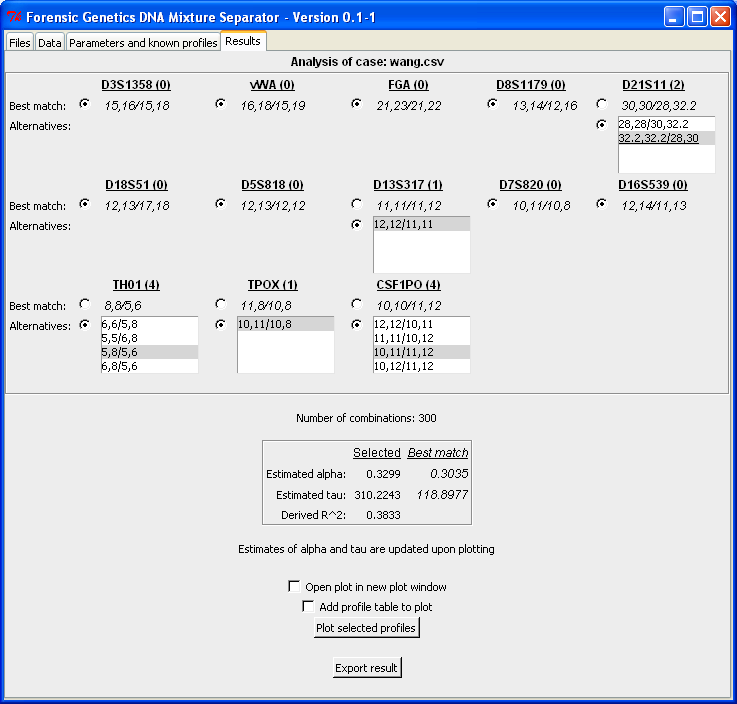
\includegraphics[width=10cm]{result_alternative}
  \caption{\label{fig:resultalt}Selecting an alternative pair of
    profiles from the list of locus-wise alternatives.}
\end{figure}

In the EPG-plot of Figure~\ref{fig:plotalt} we see a change in the fit
between the black lined cones and coloured cones. In addition to the
plot it is possible to export the results to a ASCII text file by
clicking ``Export results''. For this example the text file is printed
on page~\pageref{page:example}.

\newpage\phantom{emptyspace}\newpage

\begin{example}
  \label{page:example}
MixSep Output

Analysis of case file: wang.csv 

==== PROFILES ====

             D3S1358       vWA           FGA           D8S1179      
Best match   15,16/15,18*  16,18/15,19*  21,23/21,22*  13,14/12,16* 
Alternatives                                                        
                                                                    
                                                                    
                                                                    
             D21S11            D18S51        D5S818        D13S317      
Best match   30,30/28,32.2     12,13/17,18*  12,13/12,12*  11,11/11,12  
Alternatives 28,28/30,32.2                                 12,12/11,11* 
             32.2,32.2/28,30*                                           
                                                                        
                                                                        
             D7S820       D16S539       TH01      TPOX         CSF1PO       
Best match   10,11/10,8*  12,14/11,13*  8,8/5,6   11,8/10,8    10,10/11,12  
Alternatives                            6,6/5,8   10,11/10,8*  12,12/10,11  
                                        5,5/6,8                11,11/10,12  
                                        5,8/5,6*               10,11/11,12* 
                                        6,8/5,6                10,12/11,12  
=== PARAMETERS ===

             alpha  tau      R2    
Best match   0.3035 118.8977       
Selected (*) 0.3299 310.2243 0.3833


==== SETTINGS ====

Number of contributors: 2 
Level of significance: 0.001 
Number of combinations: 300 
\end{example}

\begin{figure}[!h]
  \centering
  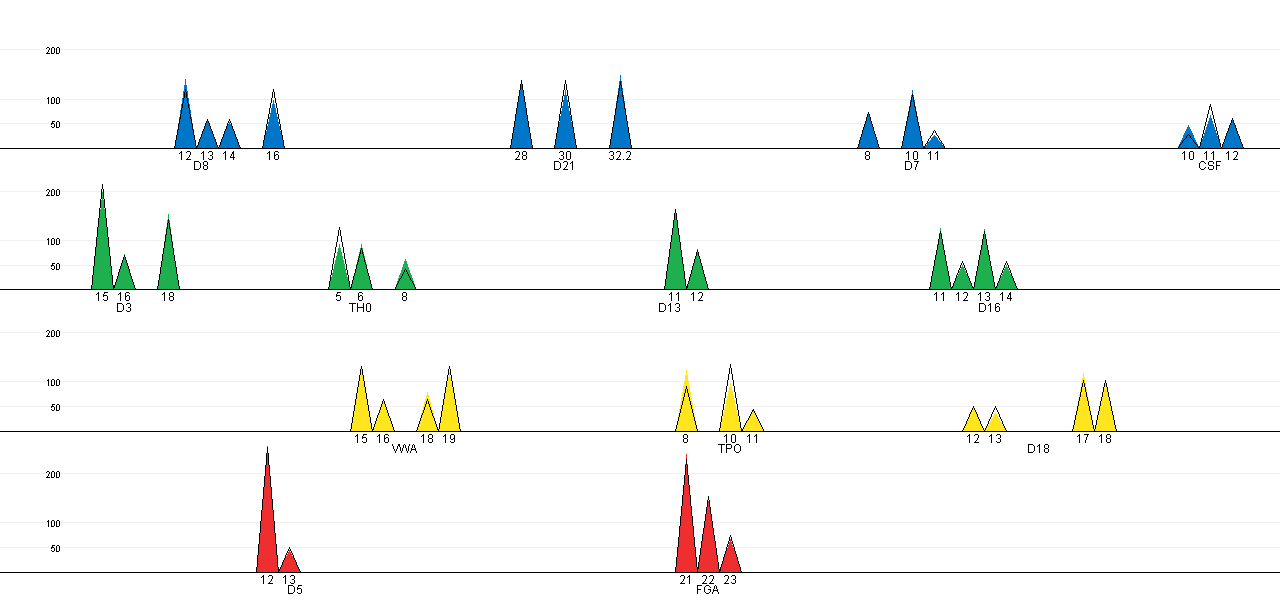
\includegraphics[width=15cm]{plot_alternative}
  \caption{\label{fig:plotalt}EPG of the alternative configuration
    specified in Figure~\ref{fig:resultalt}.}
\end{figure}

\section{Analysis with a fixed profile}
\label{sec:wangfix}

For the initial steps of loading data files and selecting columns/rows
for further analysis, please see Section~\ref{sec:wangbm} for a guide
for determining the best matching configuration). In this guide we
demonstrate how to analyse the same sample using a fixed
(e.g. suspect) profile.

The ``Parameters and known profiles''-tab makes it possible to specify
the number of contributors, whether the algorithm should search for
alternatives and fixed/known profiles. We assume the sample is a
two-person mixture and searches for alternatives (the lower the level
of significance is, the more alternatives are included in the final
result). Furthermore, we want to investigate whether the profile in
Table~\ref{tab:suspect} a possible contributor to the DNA mixture (see
parameter settings in the left screen shot of
Figure~\ref{fig:paramsuspect}).

\begin{table}[!h]
  \caption{\label{tab:suspect}DNA profiles of the true offender and the suspect
  used in the example. The bold font alleles in the suspect's profile
  denote the difference from the true offender profile (the major profile).}
{\setfontsize{10pt}
  \begin{tabular}{!{$\!\!\!$}l!{$\!\!\!\!$}*{13}{c!{$\!\!\!$}}}
  \toprule
\textbf{Locus} & \textbf{D3}& \textbf{vWA}& \textbf{FGA}& \textbf{D8}&
\textbf{D21}& \textbf{D18}& \textbf{D5}& \textbf{D13}& \textbf{D7}&
\textbf{D16}& \textbf{TH01}& \textbf{TPOX}& \textbf{CFS}\\
\midrule
Offender & 15,18& 15,19& 21,22& 12,16& 28,32.2& 17,18& 12,12& 11,12& 8,10& 11,13& 5,6& 8,10& 11,12\\
Suspect & 15,18& 15,19& 21,22& 12,16& 28,32.2& 17,18& 12,12&11,\textbf{11}& 8,10& 11,13& 5,\textbf{8}& 8,10& \textbf{12},12\\
\bottomrule
\end{tabular}%
}
\end{table}

\begin{figure}[!h]
  \centering
      \begin{tabular}{cc}
      \parbox[b]{7.5cm}{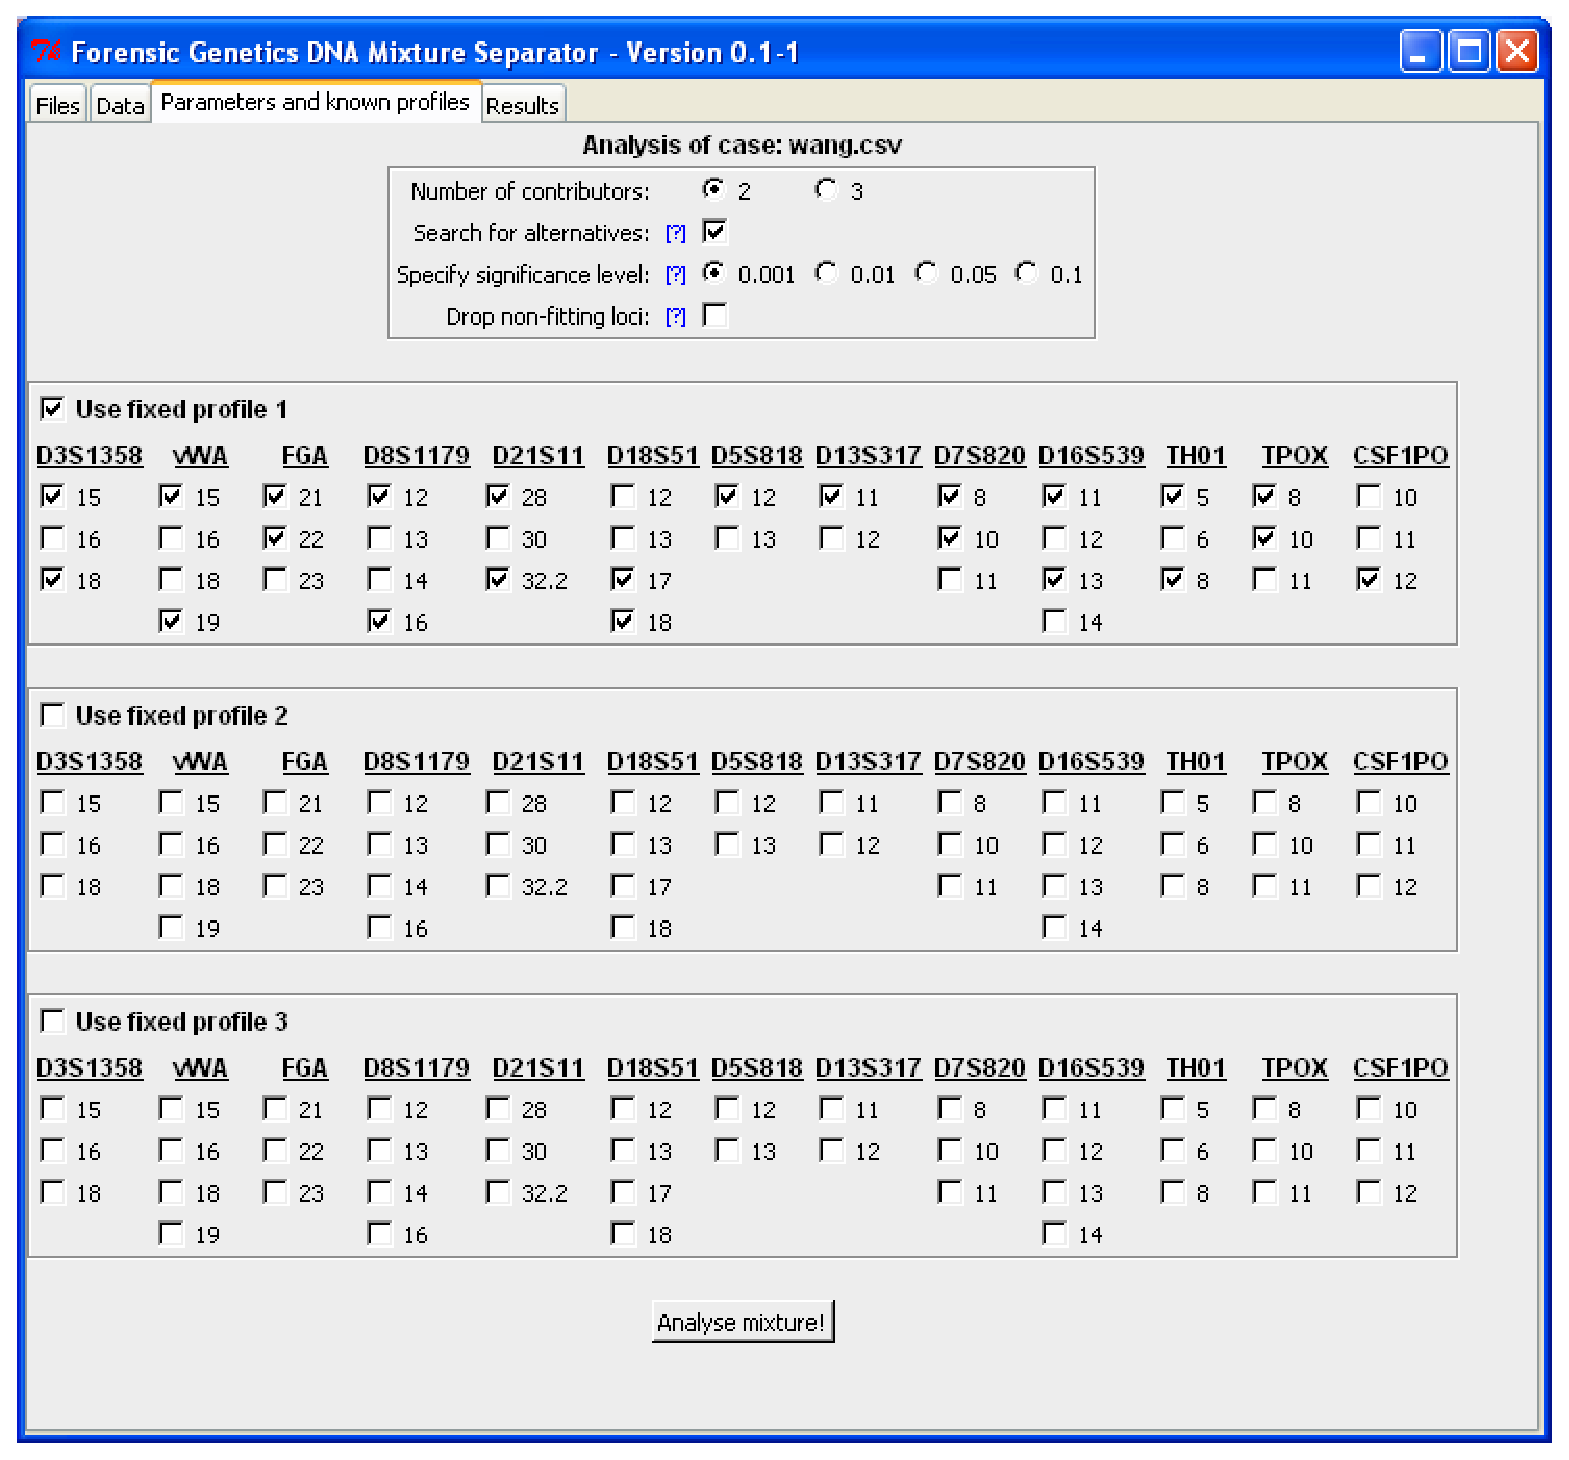
\includegraphics[width=7.5cm]{param_suspect}}
      \parbox[b]{7.5cm}{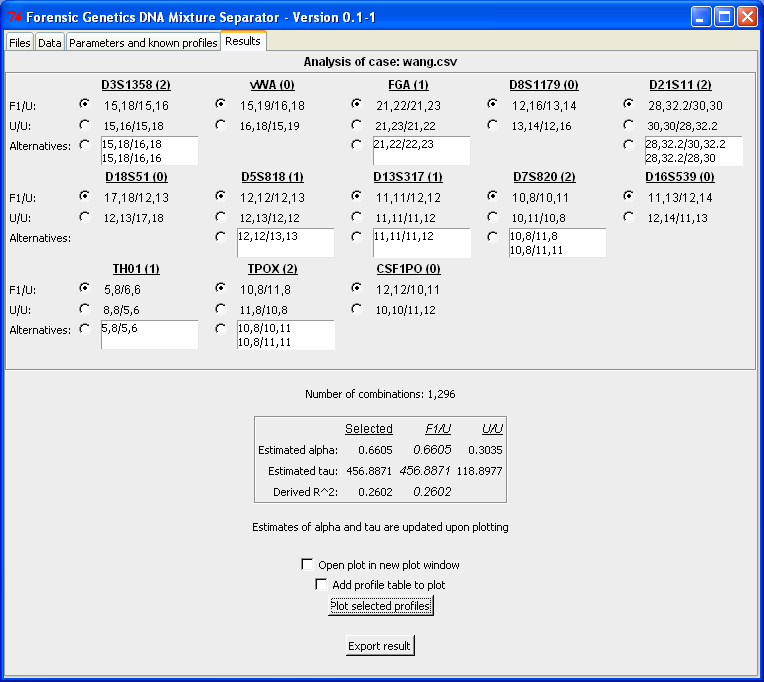
\includegraphics[width=7.5cm]{result_suspect}}
      \end{tabular}
      \caption{\label{fig:paramsuspect}Parameter settings assuming a
        two-person DNA mixture with a known/fixed contributor as
        specified by the tick-boxes.}
\end{figure}

When clicking ``Analyse mixture!'' the computer resolves the DNA
mixture and returns result in the ``Result''-tab. In the right screen
shot of Figure~\ref{fig:paramsuspect} is the output from the
analysis. For each locus the unknown profile that together with the
fixed profile best explains the DNA mixture is identified (denoted
F1/U for Fixed profile~1 and Unknown). In the U/U-row is the best
matching configurations (both profiles unspecified, i.e. U/U is short
for Unknown/Unknown). Furthermore, below is a list of possible
alternative configurations including the fixed profile.

Next to the locus designation is the number of possible alternatives
for that locus given in parenthesis. Below the list of locus
configurations is the number of total configurations given together
with the estimated parameters of the statistical model. The ``Estimated
alpha'' for F1/U represents the mixture proportion of the
\underline{fixed} contributor, whereas for U/U it denotes the
contribution from the \underline{minor} contributor. Here alpha is
respectively 0.66 and 0.3, which approximately corresponds to an
1:2-mixture ratio in both cases. The ``Estimated tau'' value represents
that residual variance, which means that the smaller the estimate the
better is the concordance between the observed and expected peak
intensities. The ``Derived R\^{}2'' is computed as the tau for U/U to
tau for F1/U. Here R\^{}2 = 0.26 = 118/457 implying that the
residual variance is four times bigger when the suspect's profile is
assumed in the mixture compared to the best matching pair (which is
identical to the true contributors, see Section~\ref{sec:wangbm}).

The expected peak intensities for the selected configuration can be
plotted against the observed peak intensities in a EPG-like plot. The
coloured cones represents the observed peak intensities, while the
black lined cones show the expected peak intensities
(Figure~\ref{fig:plotsuspect}). Note that the configuration on CSF
causes the expected peak intensities to deviate from the
observed. This is also the only combination of the three changes
between the true offender and suspect (see Table~\ref{tab:suspect}),
that is not among the alternatives in the best matching analysis (see
the results of best matching analysis in Section~\ref{sec:wangbm} -
where it should be remembered that the suspect corresponds to the
major profile).

\begin{figure}[!h]
  \centering
  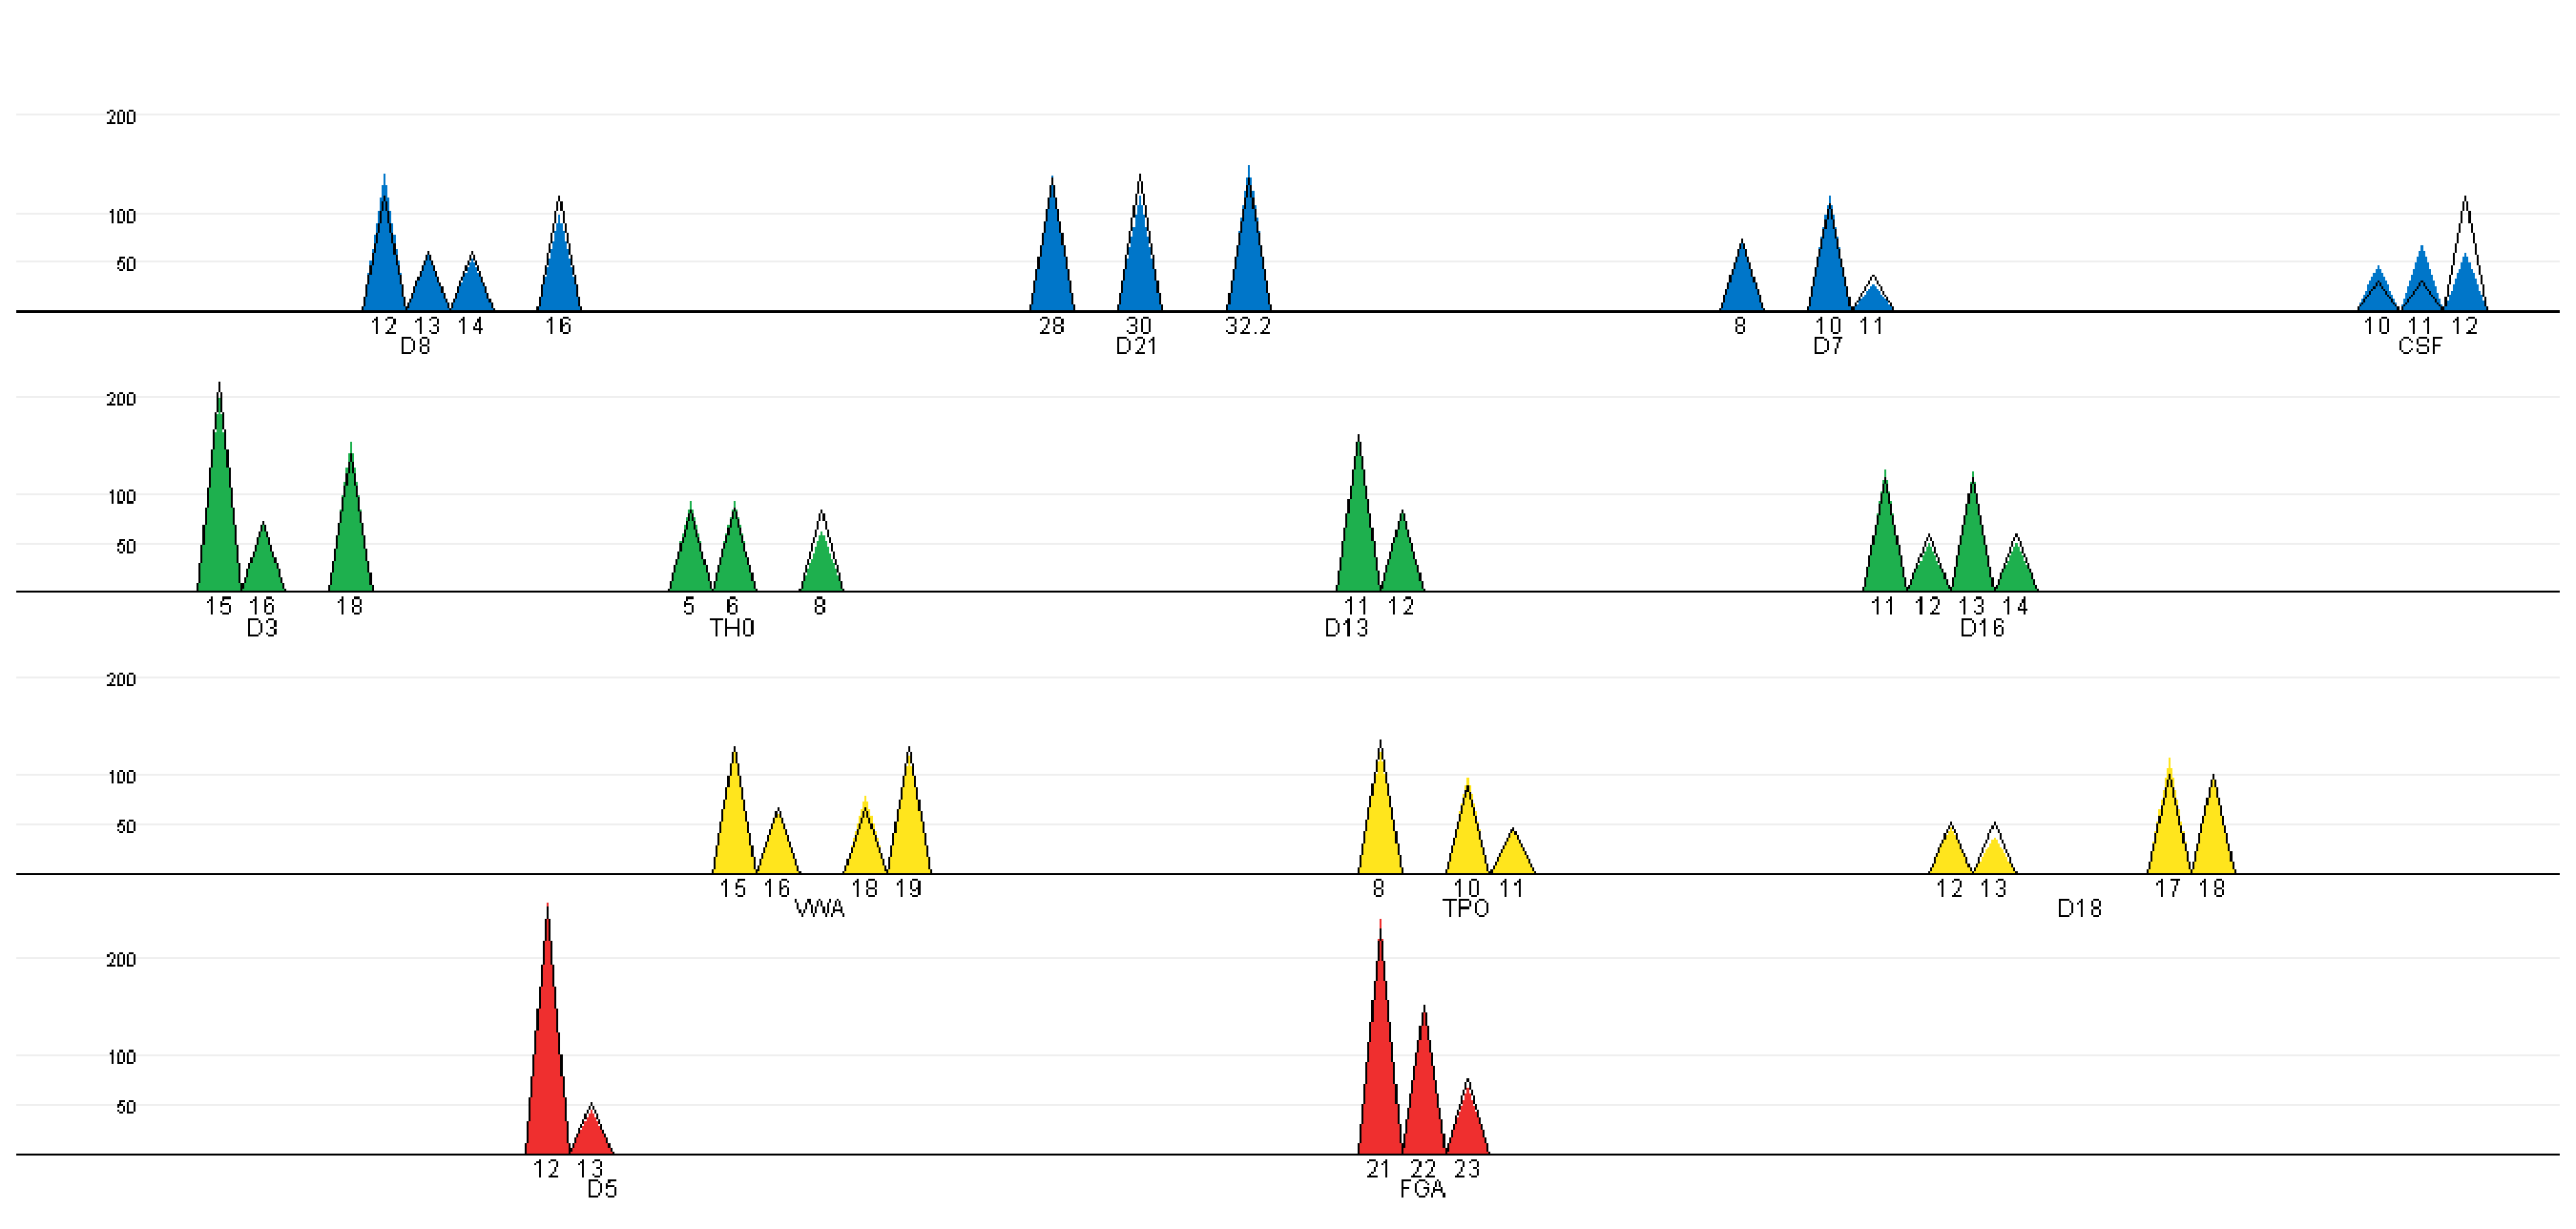
\includegraphics[width=15cm]{plot_suspect}
  \caption{\label{fig:plotsuspect}EPG with the suspect and best
    matching unknown DNA profile.}
\end{figure}

From the analysis output alternative configurations can be specified
by marking the combinations in the lists. For each locus the list of
alternatives is sorted in decreasing order in terms of
goodness-of-fit. For the selected configuration the R\^{}2 quantity is
computed as the ratio of the estimated tau values of the best matching
(U/U) and the selected configuration. In
Figure~\ref{fig:resultsuspectalt} the R\^{}2 = 0.06 = 118/2055 and the
closer R\^{}2 is to 1, the better is the alternative configuration
relative to the best match pair of profiles.

\begin{figure}[!h]
  \centering
  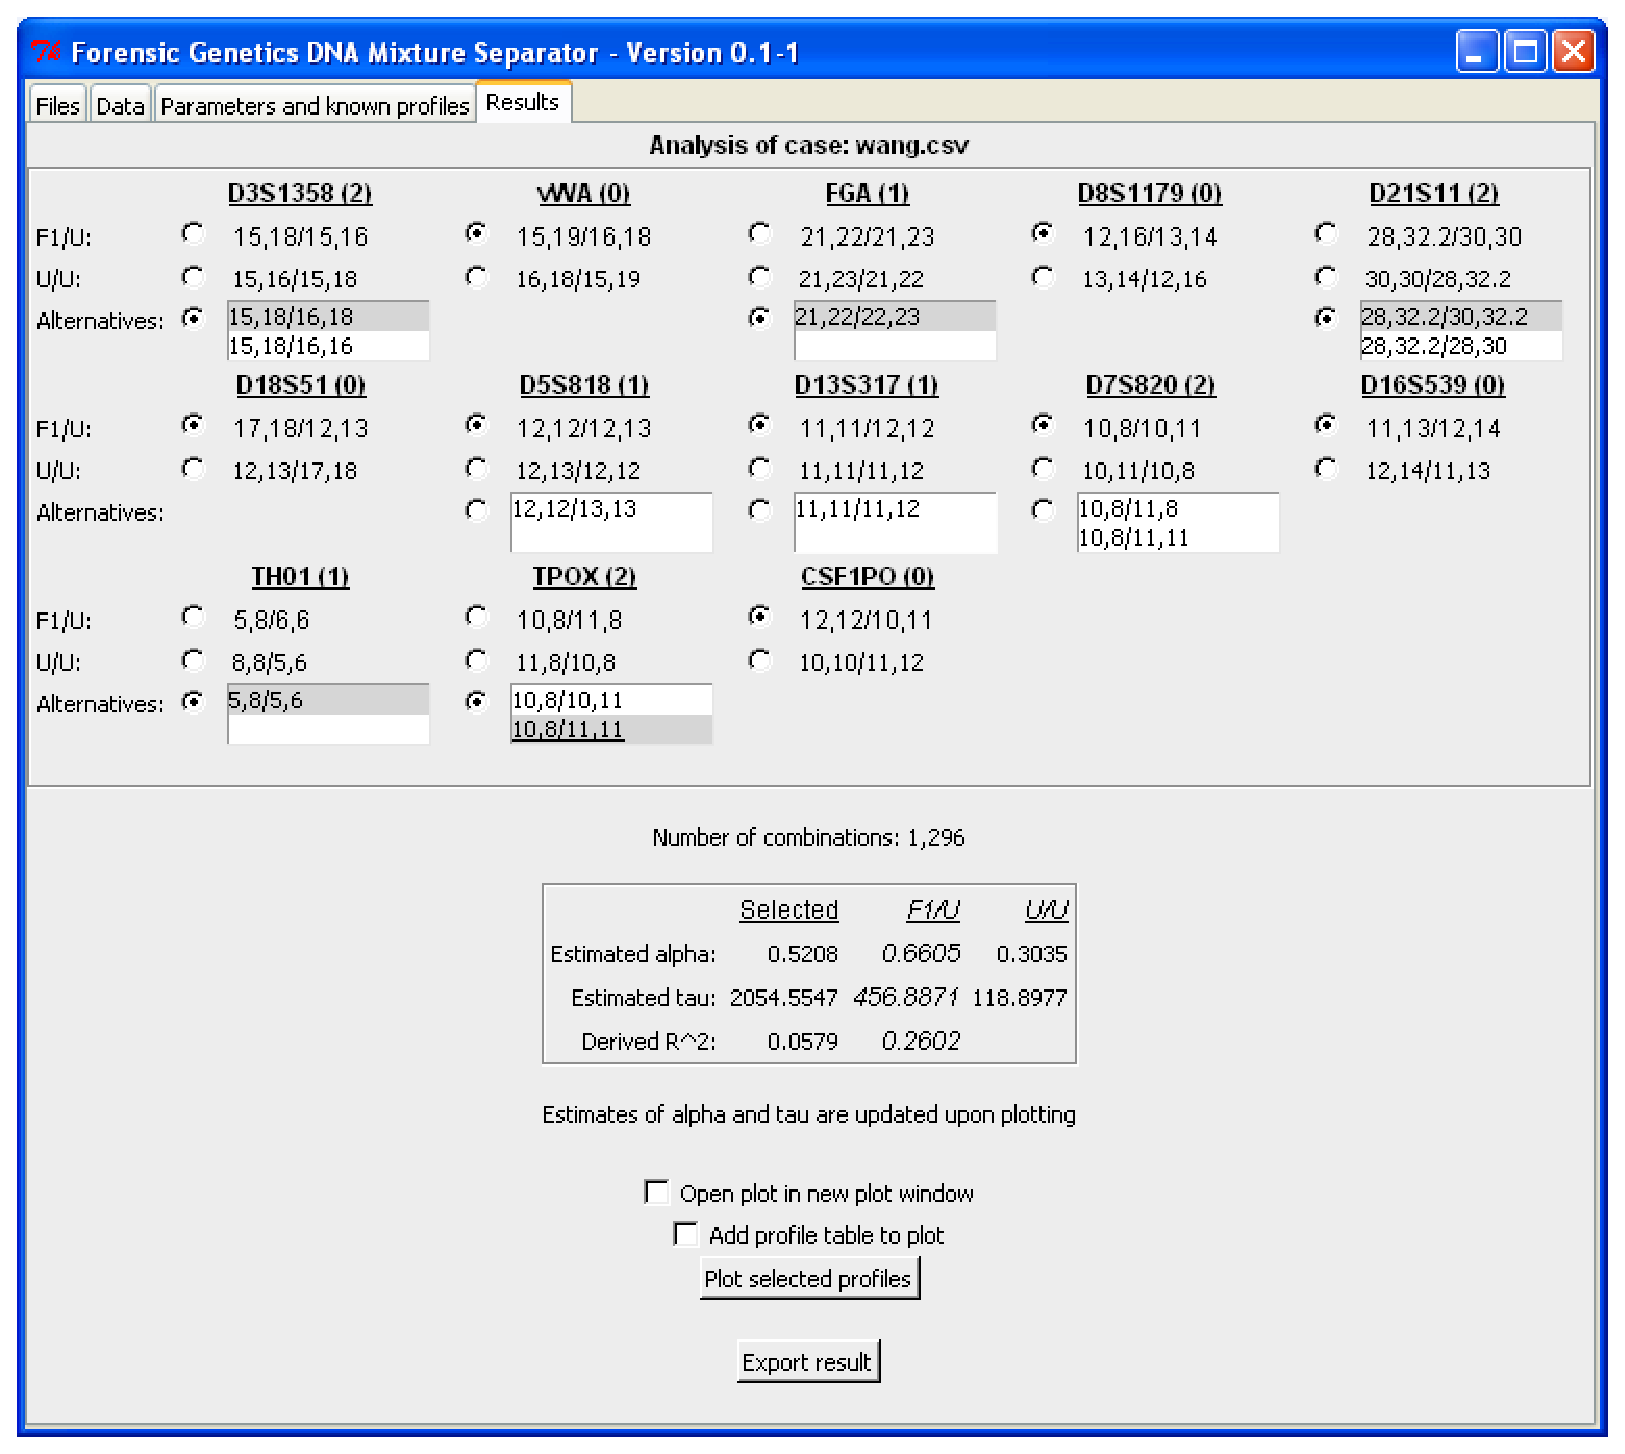
\includegraphics[width=10cm]{result_suspectalternative}
  \caption{\label{fig:resultsuspectalt}Specifying a different
    configuration (still involving the suspect).}
\end{figure}

In the EPG-plot in Figure~\ref{fig:plotsuspectalt} we see a change in
the fit between the black lined cones and coloured cones. The low
value of R\^{}2 is indicates a poor fit between the observed and
expected peak intensities, which is pictured in
Figure~\ref{fig:plotsuspectalt}. In addition to the plot it is
possible to export the results to a ASCII text file by clicking
``Export results'' as in Section~\ref{sec:wangbm}.

\begin{figure}[!h]
  \centering
  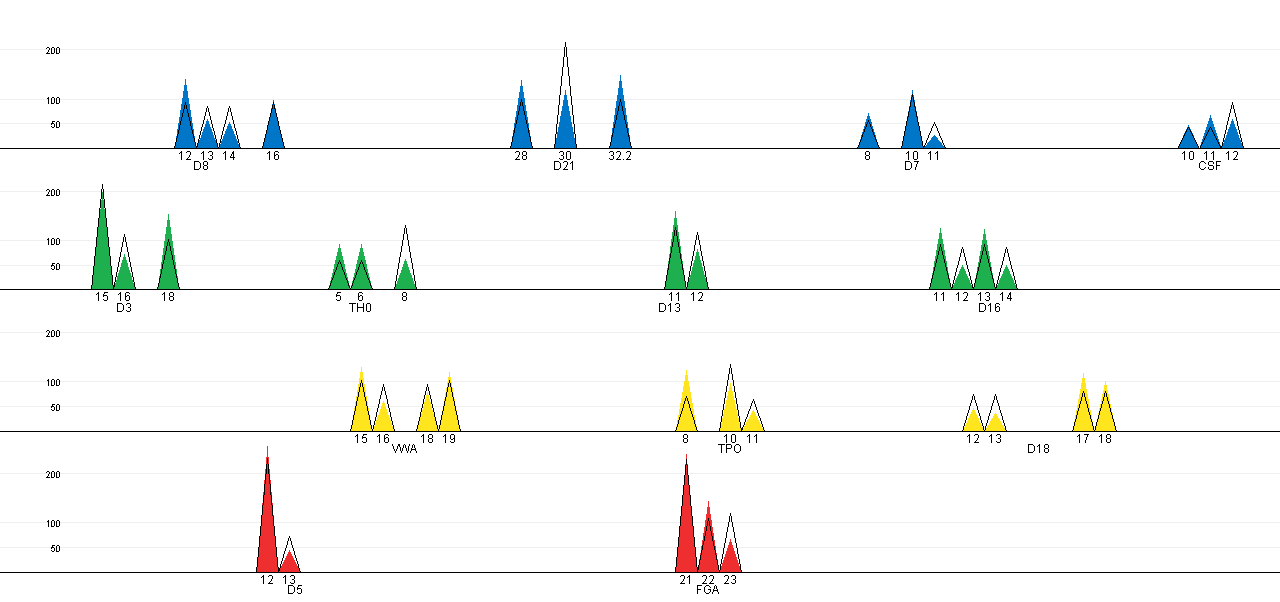
\includegraphics[width=15cm]{plot_suspectalternative}
  \caption{\label{fig:plotsuspectalt}EPG of the configuration
    specified in Figure~\ref{fig:resultsuspectalt}.}
\end{figure}

\appendix

\section{Screen shots of basic R procedures}
\label{sec:basicR}

\begin{figure}[!h]
  \centering
  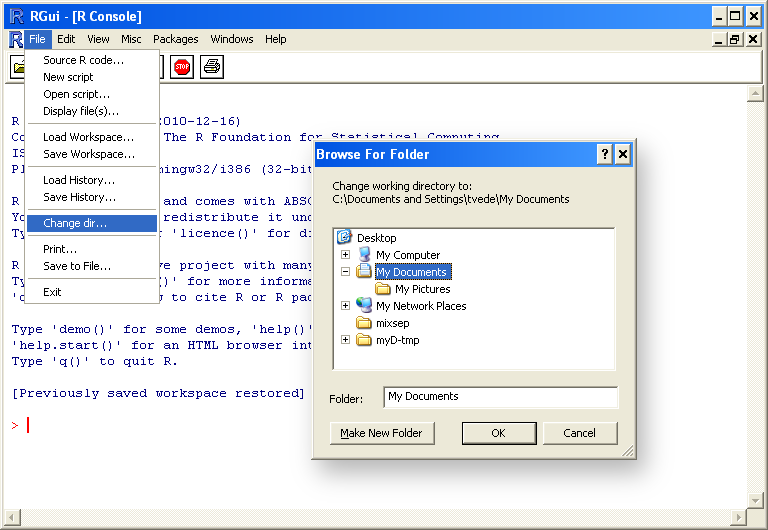
\includegraphics[width=10cm]{changedir}  
  \caption{\label{fig:changedir}Changing the working directory in the
    R Gui on Windows.}
\end{figure}

\begin{thebibliography}{}
\bibitem[\protect\citeauthoryear{Wang et al.}{Wang et
    al.}{2006}]{wang2006} 
  T.~Wang, N.~Xue, J.~D. Birdwell (2006).
  \newblock Least-Square Deconvolution: A Framework for Interpreting
  Short Tandem Repeat Mixtures.  
  \newblock Journal of Forensic Science
  51~(6) (2006) 1284--1297.
  \newblock DOI:~\href{http://dx.doi.org/10.1111/j.1556-4029.2006.00268.x}{10.1111/j.1556-4029.2006.00268.x}

\bibitem[\protect\citeauthoryear{Tvedebrink et al.}{Tvedebrink et
    al.}{2011}]{tvedebrink2011} 
  T.~Tvedebrink, P.S.~Eriksen, H.S.~Mogensen, N.~Morling (2011).
  \newblock Identifying contributors of DNA mixtures by means of
  quantitative information of STR typing.
  \newblock Computational Biology~(In Press).
  \newblock Link:~\href{http://www.liebertonline.com/doi/abs/10.1089/cmb.2010.0055}{http://www.liebertonline.com/doi/abs/10.1089/cmb.2010.0055}
\end{thebibliography}

\end{document}
